\documentclass[12pt,oneside]{report}

\usepackage[utf8]{inputenc}
\usepackage{graphicx}
\usepackage{csquotes}
\usepackage{lipsum}
\usepackage{microtype}
\usepackage{adjustbox}
\usepackage{url}
\usepackage{array}
\newcolumntype{P}[1]{>{\centering\arraybackslash}p{#1}}
\newcolumntype{M}[1]{>{\centering\arraybackslash}m{#1}}

% Packages for code style
\usepackage{minted}
\usepackage{mdframed}
\definecolor{bg-grey}{rgb}{0.95,0.95,0.95}
\usepackage{float}
\renewcommand{\figurename}{Figura}
\renewcommand{\tablename}{Tabelul}
\setlength{\belowcaptionskip}{-10pt}


% Document table of contents configuration
\usepackage{tocloft}
\cftsetindents{section}{0em}{2em}
\cftsetindents{subsection}{0em}{4em}
\renewcommand{\cftsecleader}{\cftdotfill{\cftdotsep}}
\renewcommand{\contentsname}{Cuprins}
\renewcommand\cftchapafterpnum{\vskip10pt}
\renewcommand\cftsecafterpnum{\vskip2pt}
\renewcommand\cftsubsecafterpnum{\vskip2pt}
  
% Document geometry configuration
\usepackage[
	a4paper,
	textwidth={400pt}
]{geometry}

% Hyphenation
\hyphenation{con-fi-gu-ra-bil}

\graphicspath{ {images/} }

\newenvironment{bottompar}{\par\vspace*{\fill}}{\clearpage}

\newcommand{\GLOBALDATE}{3 Iulie 2017}
\newcommand{\chaptertitle}[1]{\LARGE{#1}}

\renewcommand{\bibname}{\LARGE{Bibliografie}}
\renewcommand{\thesection}{\arabic{section}}

\begin{document}

% Pagina coperta

\titlepage{
	\begin{center}
	\large{UNIVERSITATEA \enquote{ALEXANDRU IOAN CUZA} DIN IAȘI} \\
	\vspace{0.5cm}
	\large{\textbf{FACULTATEA DE INFORMATICĂ}} \\
      \vspace{1cm}
    
\includegraphics[width=2cm,height=3cm,keepaspectratio]{sigla-fii.png}\\
	\vspace{1cm}
	\large{\textbf{LUCRARE DE LICENȚĂ}}\\
	\vspace{1cm}
	\LARGE{Surf} \\
	\vspace{0.5cm}
	\large{\textit{Parcurgere și procesare distribuită a paginilor web în cloud pentru extragerea informațiilor}} \\
	\vspace{1cm}
	\large\textbf{{propusă de}}\\ 
	\vspace{0.5cm}
	\large{\textbf{\textit{Ovidiu Pricop}}}\\
	\vspace{2cm}
	\large{\textbf{Sesiunea:} Iulie, 2017}\\
	\vspace{2cm}
	\large{\textbf{Coordonator științific}}\\
	\vspace{0.5cm}
	\large{\textbf{Conf. dr. Sabin Corneliu Buraga}}
	\end{center}
}

% Pagina titlu

\titlepage{
	\begin{center}
	\large{UNIVERSITATEA \enquote{ALEXANDRU IOAN CUZA} DIN IAȘI} \\
	\vspace{0.5cm}
	\large{\textbf{FACULTATEA DE INFORMATICĂ}} \\
    \vspace{4cm}
	\LARGE{Surf} \\
	\vspace{3cm}
	\large{\textbf{\textit{Ovidiu Pricop}}}\\
	\vspace{2cm}
	\large{\textbf{Sesiunea:} Iulie, 2017}\\
	\vspace{3cm}
	\large{\textbf{Coordonator științific}}\\
	\vspace{0.5cm}
	\large{\textbf{Conf. dr. Sabin Corneliu Buraga}}
	\end{center}
}

% Declaratie originalitate

\chapter*{
	\large{
		Declarație privind originalitate și respectarea drepturilor de autor
	}
}
Prin prezenta declar c\u{a} lucrarea de licen\c{t}\u{a} cu titlul  \enquote{Surf} este scris\u{a} de mine \c{s}i nu a mai fost prezentat\u{a} niciodat\u{a} la o alt\u{a} facultate sau institu\c{t}ie de \^{i}nv\u{a}\c{t}\u{a}m\^{a}nt superior din \c{t}ar\u{a} sau str\u{a}in\u{a}tate. De asemenea, declar c\u{a} toate sursele utilizate, inclusiv cele preluate de pe Internet, sunt indicate \^{i}n lucrare, cu respectarea regulilor de evitare a plagiatului:

\begin{itemize}
	
	\item {toate fragmentele de text reproduse exact, chiar \c{s}i \^{i}n traducere proprie din alt\u{a} limb\u{a}, sunt scrise \^{i}ntre ghilimele \c{s}i de\c{t}in referin\c{t}a precis\u{a} a sursei;}
	      
	\item {reformularea \^{i}n cuvinte proprii a textelor scrise de c\u{a}tre al\c{t}i autori de\c{t}ine referin\c{t}a precis\u{a};}
	      
	\item {codul surs\u{a}, imaginile etc. preluate din proiecte open-source sau alte surse sunt utilizate cu respectarea drepturilor de autor \c{s}i de\c{t}in referin\c{t}e precise;}
	      
	\item {rezumarea ideilor altor autori precizeaz\u{a} referin\c{t}a precis\u{a} la textul original.}
	
\end{itemize}

\begin{bottompar}
	\begin{flushleft}
		Ia\c{s}i, \GLOBALDATE
	\end{flushleft}

	\vspace{0.5cm}
	\begin{flushright}
		Ovidiu Pricop
	\end{flushright}
\end{bottompar}

% Declaratie consimtamant

\chapter*{
	\large{
		Declarație de consimțământ
	}
}
Prin prezenta declar c\u{a} sunt de acord ca Lucrarea de licen\c{t}\u{a} cu titlul \enquote{Surf}, codul surs\u{a} al programelor \c{s}i celelalte con\c{t}inuturi (grafice, multimedia, date de test etc.) care \^{i}nso\c{t}esc aceast\u{a} lucrare s\u{a} fie utilizate \^{i}n cadrul Facult\u{a}\c{t}ii de Informatic\u{a}.
De asemenea, sunt de acord ca Facultatea de Informatic\u{a} de la Universitatea Alexandru Ioan Cuza Ia\c{s}i s\u{a} utilizeze, modifice, reproduc\u{a} \c{s}i s\u{a} distribuie \^{i}n scopuri necomerciale programele-calculator, format executabil \c{s}i surs\u{a}, realizate de mine \^{i}n cadrul prezentei lucr\u{a}ri de licen\c{t}\u{a}.

\begin{bottompar}
	\begin{flushleft}
		Ia\c{s}i, \GLOBALDATE
	\end{flushleft}

	\vspace{0.5cm}
	\begin{flushright}
		Ovidiu Pricop
	\end{flushright}
\end{bottompar}

% Rezumat

\chapter*{\chaptertitle{Rezumat}}
\addcontentsline{toc}{chapter}{Rezumat}
La nivelul internetului, traficul global a crescut de aproximativ 850 de ori in perioada 2000 - 2015 \cite{cisco-internet-traffic}. World wide web-ul reprezinta o parte semnificativa a volumului de informatii interschimbate pe internet. In anul 2015 existau peste jumatate de miliard de situri web accesibile \cite{http://www.internetlivestats.com/total-number-of-websites/}. Fiecare pagina web raspunde anumitor nevoi (sociale, financiare, educationale etc.). O singura sursa de informatii este uneori suficienta pentru a raspunde nevoilor unui utilizator. Alteori, este necesar un ansamblu de surse informative (e.g. newsletter-e zilnice din 5 surse diferite), pentru a urmari un subiect din mai multe perspective sau a-i intregi continutul.
\\
\\
Prezenta lucrare urmareste elaborarea unui serviciu web distribuit in cloud pentru parcurgerea, selectarea, colectarea si indexarea informatiilor la nivelul world wide web-ului.

\newpage


% Cuprins

\tableofcontents
\clearpage

% Introducere
\chapter*{\chaptertitle{Introducere}}
\addcontentsline{toc}{chapter}{Introducere}
\newcommand{\xmlDescription}{Extensible Markup Language - https://www.w3.org/XML/}
\newcommand{\jsonDescription}{JavaScript Object Notation - http://www.json.org/}
\newcommand{\crawlDescription}{https://en.wikipedia.org/wiki/Web\_crawler}

Un serviciu web reprezinta o componenta functionala ce indeplineste anumite sarcini. Comunicarea cu un serviciu web se realizeaza independent de platforma, limbajul de programare sau sistemul de operare pe care este dezvoltat. Schimbul de informatii se realizeaza prin mesaje text ce respecta un format standardizat precum xml\footnote{\xmlDescription} sau json\footnote{\jsonDescription}. 
\\
\\
Aplicatia "Surf" reprezinta un serviciu web specializat in web crawling\footnote{\crawlDescription}, dezvoltat folosind tehnologii cloud din cadrul Amazon Web Services. Se urmareste crearea unui serviciu web cu disponibilitate permanenta, scalabil si de inalta putere computationala care sa orchestreze colectarea distribuita de informatii din aria definita de utilizator.
\\
\\
Comunicarea cu aplicatia "Surf" se realizeaza prin intermediul unui API Restful\footnote{https://en.wikipedia.org/wiki/Representational\_state\_transfer} construit pe platforma AWS\footnote{Amazon Web Services} API Gatway. Autentificarea utilizatorilor se va realiza printr-un serviciu OpenID Connect (e.g. Google, Facebook etc.). Autorizarea va avea ca principala componenta AWS IAM. Utilizatorilor le vor fi repartizate, in functie de privilegiile asociate cu cheia de autentificare, o serie de roluri (i.e. drepturi de access asupra resurselor din cadrul serviciului "Surf"). Executia codului propriu-zis, gazduit de functii AWS Lambda, va interactiona cu baza de date no-sql AWS DynamoDB pentru a eficientiza accesul la informatii cheie (metadate crawling, date autentificare etc.). Mediul de procesare distribuita va fi sustinut de AWS Simple Workflow Service si configurat dupa preferintele utilizatorului. Datele extrase din procesul de web-crawling vor fi salvate in mediul persistent de stocare AWS S3. Evenimentele legate de parcurgerea siturilor vor fi expuse, ca metadate, intr-o coada AWS SQS si vor fi accesibile utilizatorilor prin procesul de long-polling asupra acestei cozi.

\clearpage

% Descrierea unui crawler web
\section{Descrierea unui crawler web}
Natura dinamică World Wide Web-ului, precum şi scara sa, justifică necesitatea existenţei unor mecanisme eficiente de localizare a informaţiilor relevante. Instrumentele specializate în căutarea datelor se bazează pe web crawler-e pentru colectarea informaţiilor din paginile web, ce sunt, ulterior, indexate şi analizate.
\\ 

Crawlerul ajută utilizatorul în ceea ce priveşte navigarea Internetului, automatizând parcurgerea link-urilor. Un crawler exploatează structura web-ului şi extrage resurse, într-o manieră ordonată, ghidat de criteriile specificate de către utilizator. Rezultatul obţinut de pe urma utilizării unui web crawler este o serie de situri web.
\\

În documentele de referinţă, web crawler-ii mai sunt cunoscuţi şi drept "wanderers",  "robots", "spiders", "fish" sau "worms". Aceste denumiri nu sunt indicatori ai performanţei, întrucât aceste programe pot fi foarte rapide şi precise. Se pot parcurge zeci de mii de pagini într-un interval de câteva minute, consumând doar o fracţiune din lungimea de bandă pusă la dispoziţie \cite{GautamPadminiFilippo}, atât timp cât crawler-ul dispune de resursele hardware necesare.
\\ 

Crawler-ii web deservesc unui număr mare de scopuri. Unul dintre acestea este mentenanţa bazei de date în care sunt stocaţi indecşii unui motor de căutare. Pentru această sarcină sunt utilizaţi crawleri de tip exhaustiv (se parcurg toate siturile web întâlnite). O altă categorie este cea a crawler-ilor bazaţi pe conţinut, folosiţi pentru adunarea datelor ce se înscriu sub o anumită tematică, minimizând efortul de a aloca resurse pentru pagini irelevante. În construirea unui astfel crawler este necesară definirea unei modalităţi de căutare şi selecţie a datelor. În cazul crawlerilor bazaţi pe conţinut, pot apărea probleme legate de explorare versus exploatare, deoarece spaţiul de căutare ar putea conţine un optim local, împiedicând algoritmul să localizeze optimul global.\cite{PantSrinivasanMenczer} 
\\

\section{Design-ul unui crawler web}
Ca si design, un crawler web se rezuma la trei elemente: o \textit{frontiera}, in care sunt stocate URL-urile ce urmeaza a fi vizitate, o componenta a carei scop este de a \textit{downloada paginile} de pe World Wide Web si un spatiu de stocare, unde sa fie persistate datele preluate de la crawler (e.g. o baza de date si/sau un sistem de fisiere) \cite{Pantil, GautamPadminiFilippo}.
\\

\subsection{Frontiera}
In terminologia grafurilor, frontiera reprezinta lista nodurilor nevizitate \footnote{"[...] unexpanded (unvisited) nodes." \cite{PantSrinivasanMenczer} }. Pentru un crawler web, frontiera reprezinta o lista de likuri neparcurse. Procesul de cautare porneste de la un link numit radacina, care este preluat din web si procesat, uramand ca link-urile gasite sa fie adaugate in frontiera. Aceasta lista poate capata dimensiuni foarte mari inca de la inceputul procesului de parcurgere a paginilor, intrucat media de legaturi de pe o pagina web este 7 link-uri/pagina \footnote{"The web  may  be  viewed  as  a  directed  graph  in  which each vertex is a static HTML web page, and each edge is a hyperlink from one web page to another. Current estimates suggest that this graph has roughly a billion vertices, and an average degree of about 7."\cite{StochasticModels}}. Procesul se repeta, alegandu-se, folosind un anumit algoritm, link-uri din frontiera, pana cand frontiera se goleste sau alta conditie de oprire permite finalizarea cautarii.
\\

\subsection{Descărcarea paginilor web}
Este necesar un client HTTP care trimite o cerere HTTP si primeste un raspuns. In aceasta etapa, nu trebuie trecut cu vederea "The Robots Exclusion Standard", cunoscul si drept "Robots Exclusion Standard" sau robots.txt \cite{RobotsStandard}. Protocolul ofera administratorilor de servere web posibilitatea de a-si comunica politicile de acces si de a mentiona paginile care nu sunt destinate crawler-ilor.
\\

\subsection{Stocarea datelor}
În urma parcurgerii paginilor web, datele obținute sunt stocate într-un mediu potrivit nivelului lor de abstractizare. Spre exemplu, metadatele vor fi stocate într-un mediu în care interogarea să se poată realiza în mod eficient, iar paginile în format HTML vor fi păstrate într-un mediu de stocare mai încăpător.
\\
\clearpage

% Crawler-ul Surf
\section{Crawler-ul Surf}
\newcommand{\robotsTxtDescription}{http://www.robotstxt.org/robotstxt.html}

Ca sens general, un crawler web reprezinta un program care parcurge, prin cereri succesive, situri web. Programatic, vom considera urmatoarele aspecte cheie in proiectarea unui crawler distribuit:

\begin{enumerate}

	\item{Punctele de pornire in parcurgerea siturilor web;}
	
	\item{Adancimea maxima a parcurgerii recursive a siturilor (i.e. cea mai indepartata pagina la care se poate ajunge, de la punctul de pornire, prin accesarea succesiva a legaturilor de tipul hyperlink;}
	
	\item{Politica de selectie a informatiilor din paginile parcurse\cite{web-crawler-selection-policy};}
	
	\item{Viteza de crawling, fisierul \emph{robots.txt}\footnote{\robotsTxtDescription} si respectarea drepturilor de autor;}
	
	\item{Politica de paralelizare a procesului de web crawling;}
	
	\item{Politica de retentie temporara a rezultatelor parcurgerii siturilor web si logare a actiunilor serviciului de crawling;}
	
\end{enumerate}

In cele ce urmeaza, se va descrie particularizarea aspectelor generale enumerate mai sus in cadrul serviciului web "Surf". Se va crea, astfel, contextul dezvoltarii aplicatiei si se vor puncta principalele componente functionale implicate.


\subsection{Puncte de pornire}
\newcommand{\urlDescription}{Uniform Resource Locator - http://www.dictionary.com/browse/url, folosit, in acest context, cu sensul de identificator unic al unei resurse web}

Pentru a putea parcurge siturile web, crawler-ul "Surf" necesita unul sau mai multe puncte de pornire. Un punct de pornire este definit printr-un URL\footnote{\urlDescription} si este furnizat, ca input din partea utilizatorului, la initializarea crawler-ului.

\subsection{Parcurgere}
Crawler-ul web "Surf" are ca scop extragerea informațiilor cerute de către utilizator. Întrucat utilizatorul are posibilitatea de a furniza, ca punct de pornire, un sit web relevant pentru informația căutată, parcurgerea recursivă se va executa în manieră breadth-first. Așadar, crawler-ul va vizita toate legăturile de tip hyperlink din pagina curentă a parcurgerii înainte de a accesa legăturile din pagina următoare din punct de vedere ierarhic. Adâncimea maximă a arborelui de legături realizat prin parcurgerea URL-urilor va fi definită de către utilizator, la inițializarea sesiunii de crawling.

\subsection{Selecția informațiilor}
Selectia informatiilor necesita parcurgerea siturilor web aflate la adresele URL pe care crawler-ul le are in vedere, parsarea informatiilor in functie de tipul lor (e.g. html, xml, json, text) si extragerea blocurilor de continut aferente.
\\
\\
Un "bloc de continut" asociat unui URL reprezinta o parte a intregului continut aflat la URL-ul respectiv, filtrata dupa anumite caracteristici stabilite de utilizatorul serviciului web. Aceste caracteristici pot fi:

\begin{itemize}
	\item{Pentru fisiere HTML/XML:
		\begin{itemize}
			\item{selectori CSS/jQuery}
			\item{cuvinte cheie}
			\item{o combinatie logica a punctelor de mai sus (e.g. toate tagurile \textless{}p\textgreater{ }  in care se afla cuvintele cheie "om" si "luna")}
		\end{itemize}			
	}
	\item{Pentru fisiere text:
		\begin{itemize}
			\item{cuvinte cheie}
		\end{itemize}			
	}
\end{itemize}

\noindent
Pentru tipurile de continut enumerate mai sus sau pentru alte tipuri de continut aflate la adresele URL vizitate de crawler, utilizatorul poate defini filtre bazate pe continutul textual al URL-ului. Spre exemplu, se pot evita toate URL-urile care nu satisfac o anumita expresie regulata sau un anumit tip de continut  MIME\footnote{https://en.wikipedia.org/wiki/Media\_type} (e.g. "image/png"). 
\\
\\
Evitarea selectarii informatiilor duplicate se amelioreaza prin normalizarea\footnote{https://en.wikipedia.org/wiki/URL\_normalization} URL-urilor parcurse de catre "crawler".


\subsection{Viteză, politici de respingere și drepturi de autor}
\newcommand{\blacklistingDefinition}{http://dictionary.cambridge.org/dictionary/english/blacklist}
\newcommand{\tosDefinition}{http://www.pcmag.com/encyclopedia/term/62682/terms-of-service}

Siturile web pot implementa variate modalitati de contracarare a incercarilor de crawling. Aplicatia "Surf" incearca sa minimizeze riscul de respingere a cererilor de accesare a anumitor resurse web printr-o implementare neintruziva a procesului de crawling. Cateva aspecte esentiale care sunt luate in considerare in ceea ce priveste o astfel de implementare sunt urmatoarele:

\begin{itemize}

	\item{Minimizarea volumului de date preluat de pe un anumit domeniu prin diferite metode de filtrare a linkurilor urmarite (e.g. o anumita structura a URL-ului, un anumit tip de date care se gaseste la URL-ul respectiv);}
	
	%\item{Introducerea pauzelor temporale aleatoare intre accesari succesive a datelor apartinand aceluiasi domeniu.}
	
\end{itemize}

\noindent
Crawler-ul web "Surf" poate satisface numeroase cerinte ale utilizatorilor. O parte dintre aceste cerinte poate veni din partea sistemelor anti-malware. In acest caz, nu se doreste respectarea fisierului \emph{robots.txt} (utilizat drept referinta, pentru crawleri, asupra URL-urilor accesibile ale domeniului vizitat), deoarece exista pericolul ca un sit malitios sa blocheze o eventuala scanare. De aceea, aplicatia "Surf" va putea fi configurata in ceea ce priveste ignorarea fisierului \emph{robots.txt} in procesul de parcurgere a unui domeniu.
\\
\\
Crawler-ul "Surf" implementeaza un mecanism de \emph{blacklisting}\footnote{\blacklistingDefinition}. Siturile web sau domeniile care interzic procesul de crawling (e.g. prin ToS\footnote{\tosDefinition}) vor fi adaugate unei liste de excluziune din procesul de parcurgere executat de crawler.


\subsection{Paralelizare}
\hyphenation{statica}
"Surf" implementează un mecanism de crawling distribuit. Mai exact, există posibilitatea de a împărți sarcinile de parcurgere a paginilor web prin rularea concurentă a mai multor instanțe de funcții Lambda\footnote{\textit{Amazon Web Services Lambda Functions}:Pe baza principiilor programării funcționale, se garantează că funcțiile \textit{Lambda} nu au efecte colaterale, deci nu pot schimba starea globală a sistemului. Din acest motiv, funcțiile \textit{Lambda} se pretează la paralelizare}.
\\
\\
Există doua moduri bine cunoscute de alocare a sarcinilor de web crawling: statică și dinamică\cite{distribution-of-crawling-tasks}. Aplicația "Surf" implementează un mecanism de distribuire statică a sarcinilor:
\begin{quote}
	Fie \emph{n}, \emph{gradul de paralelizare}\footnote{Numărul maxim de execuții simultane de sarcini de crawling} configurat pentru execuția curentă a web crawler-ului. Alocarea statică va asocia fiecărui URL candidat pentru crawling un număr întreg în intervalul [1,\emph{n}] reprezentând identificatorul uneia dintre cele \emph{n} instanțe paralele ale web crawler-ului. Sarcina va fi distribuită pe acea instanță și va fi executată.
\end{quote}


\subsection{Logarea acțiunilor și retenția datelor}
In timpul executiei, crawler-ul genereaza evenimente ce sunt adaugate la istoricul executiei curente. Aceste evenimente sunt utile, in primul rand, in cazul in care executia instantei curente a crawler-ului esueaza. Sarcinile de crawling web pot dura o perioada considerabila si nu este dezirabila refacerea intregului proces de parcurgere a siturilor, atat timp cat exista rezultate partiale; executia se poate relua pornind de la ultimul eveniment valid inregistrat in istoric.  In al doilea rand, istoricul este util pentru utilizator, deoarece il poate avertiza in legatura cu statutul executiei curente a web crawler-ului.
\\
\\
Datele rezultate in urma procesului de crawling al paginilor web sunt salvate in serviciul persistent de stocare S3, din cadrul Amazon Web Services. Deoarece aceste date pot deveni volumnioase (in functie de politica de selectie configurata), aplicatia "Surf" salveaza metadate asociate acestor rezultate intr-o tabela DynamoDB. Pe baza acestor informatii (metadate), utilizatorul are optiunea de a accesa rezultatele complete corespunzatoare rularii crawler-ului web, aflate in S3.
\clearpage

\setcounter{section}{0}
\chapter*{\chaptertitle{Crawling în cloud}}
\addcontentsline{toc}{chapter}{Crawling în cloud}
Aplicatia "Surf" este construita si ruleaza in cloud. Dezvoltarea unei aplicatii pe suportul unei infrastructuri cloud este substantial diferita fata de abordarea clasica, pe o singura masina de calcul. Cloud computing-ul pune la dispozitie, la cerere, un set de resurse (e.g. putere de procesare, spatiu de stocare) pe care un utilizator (e.g. aplicatia "Surf") le poate folosi. Faptul ca toate aceste resurse sunt administrate de fiecare serviciu cloud in parte usureaza sarcinile consumatorului: se pot solicta mai multe sau mai putine dupa gradul de incarcare al aplicatiei dezvoltate in cloud. Acest lucru se realizeaza intr-o maniera transparenta pentru utilizator, fara a necesita efort suplimentar din partea acestuia.
\\
\\
Dezvoltarea aplicatiei "Surf" folosind servicii cloud mai prezinta un avantaj considerabil, deoarece comunicarea prin internet intre componentele aplicatiei si, implicit, utilizarea unui format agnostic de arhitectura sau limbaj de programare, conduce la un grad mare de decuplare. Fiind decuplate, componentele aplicatiei pot fi construite, testate si depanate\footnote{\emph{engl.} debugged} in izolare si pot functiona ca module (plugin-uri) in alcatuirea arhitecturii sistemului.
\\
\\
A dezvolta un serviciu web folosind exclusiv tehnologii cloud permite realizarea unui sistem de subscriptii granular. Un utilizator al aplicatiei "Surf" poate solicita una sau mai multe instante ale crawler-ului care sa ruleze in paralel, in functie de necesitatile proprii. Serviciile cloud permit aplicatiei sa scaleze\footnote{https://en.wikipedia.org/wiki/Scalability} orizontal ca timp, permitand utilizatorului realizarea mai multor sarcini de parcurugere automata web (deci, in consecinta, acoperirea unui volum mai mare de informatii) in acelasi interval de timp.
\\
\\
Un alt aspect relevant in realizarea serviciului web "Surf" este caracterul sau \emph{serverless}. Infrastructura \emph{serverless} implica executia codului sursa al programului in cadrul serviciilor cloud folosite pentru dezvoltarea aplicatiei. Cererile de executie a codului sunt monetizate conform unei masuri abstracte corespunzatoare resurselor utilizate pentru satisfacerea solicitarii, ceea ce difera fata de modelul clasic, in care ar fi trebuit achizitionat hardware in acest scop\cite{serverless-characterization}.

\section{Infrastructura}
\newcommand{\AWSSTS}{Serviciu web ce permite unui utilizator sa solicite credentiale temporare pentru autentificarea in cadrul platformei Amazon Web Services}
\newcommand{\openIDDefinition}{http://openid.net/what-is-openid/}

\usemintedstyle{rrt}

Esenta aplicatiei "Surf" se afla in codul executat de serviciul web AWS Lambda, care preia componentele dezvoltate pentru crawling web si le executa drept programe autonome folosind infrastructura AWS. AWS Lambda executa acest cod doar cand este nevoie (e.g. la cererea utilizatorului care doreste sa demareze operatiunea de crawling). Se minimizeaza, astfel, atat costurile utilizatorului in ceea ce priveste rularea crawler-ului web (nu necesita hardware dedicat pentru procesarea paginilor web), cat si costurile dezvoltatorilor crawler-ului, care nu trebuie sa rezerve hardware in cloud (e.g. masini virtuale Amazon EC2, inchiriere de hosturi), ca mai apoi, cand nu exista cereri suficiente, aceste masini de calcul sa ramana nefolosite. De asemenea, se renunta la necesitatea de a avea un load-balancer care sa distribuie sarcinile de crawling pe capacitatea hardware disponibila, deoarece acest lucru este administrat, in fundal, de catre AWS Lambda.
\\
\\
Functiile programatice disponibile prin serviciul AWS Lambda pot fi accesate de catre utilizatori printr-un API Restful gazduit de AWS API Gateway. Aceasta platforma permite integrarea cererilor HTTP externe cu mecanismul de autentificare si autorizare a utilizatorilor si codul executat de instantele functiilor Lambda. De asemenea, aplicatia utilizeaza functionalitati de management, monitorizare si analiza a traficului din cadrul API-ului "Surf" care permit, printre altele, inregistrarea si monetizarea functionalitatilor oferite de serviciul web pentru fiecare utilizator in parte. 
\\
\\
Pentru a putea accesa functionalitatile oferite de API-ul "Surf", utilizatorii trebuie sa se autentifice cu un furnizor tert de identitati ce suporta OpenID\footnote{\openIDDefinition}. Credentialele obtinute sunt impachetate intr-o cerere catre AWS Security Token Service\footnote{\AWSSTS}, unde sunt validate. In cazul in care validarea este indeplinita cu succes, Security Token Service returneaza utilizatorului credentiale temporare pentru a accesa servicii din cadrul AWS. Utilizatorul trebuie sa includa aceste credentiale in fiecare cerere catre API-ul "Surf" (autentificare). Odata autentificat, utilizatorul poate interactiona doar cu acele resurse ale API-ului pentru care are drepturi de acces. 
\newpage

\begin{figure}[ht]
\begin{center}
	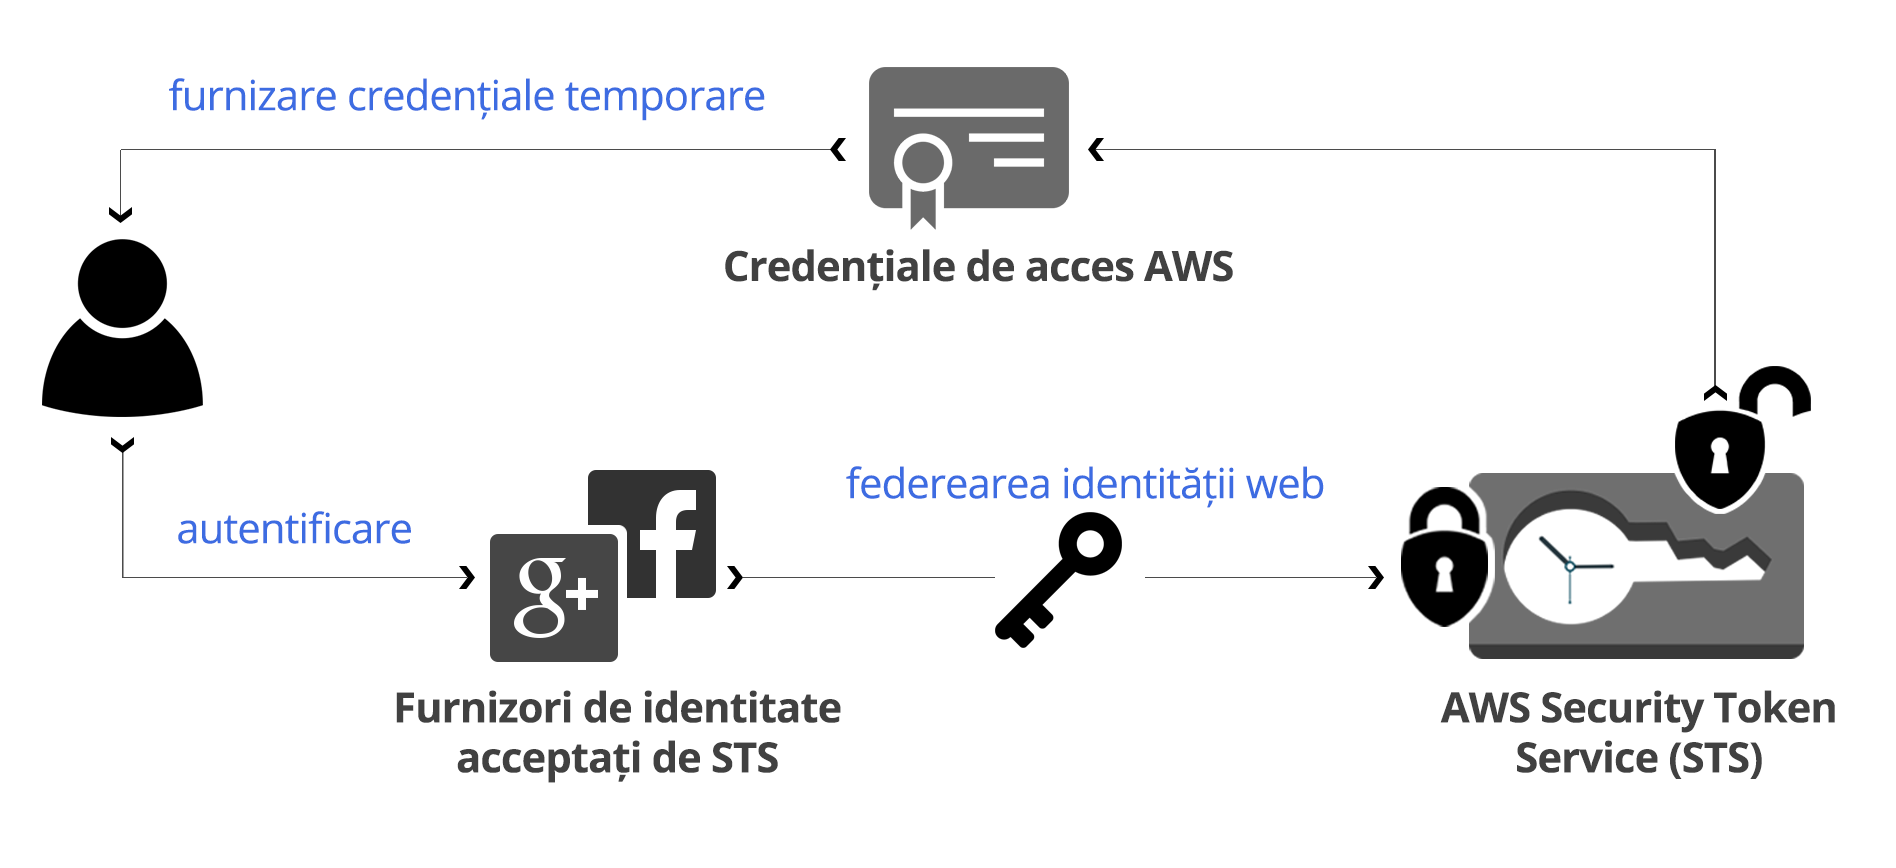
\includegraphics[keepaspectratio, width=1.0\textwidth]{obtinere-credentiale-aws.png}
	\caption{Procesul de autentificare \cite{diagram-icons-sources}}\par\medskip
	\vspace{10mm}
	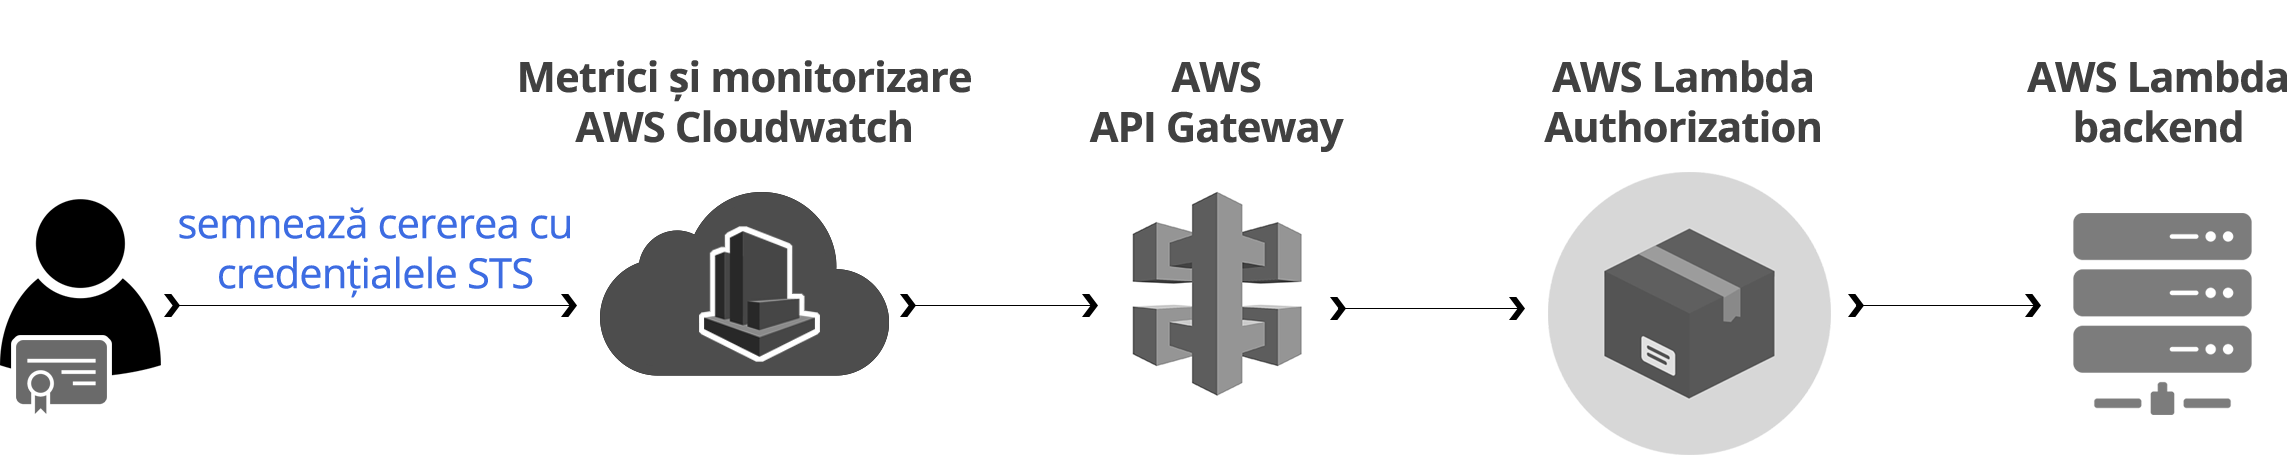
\includegraphics[keepaspectratio, width=1.0\textwidth]{autorizare.png}
	\caption{Procesul de autorizare \cite{diagram-icons-sources}}\par\medskip

\end{center}
\end{figure}

\noindent
Prin AWS Identity Access Management (IAM) se vor stabili restrictiile de acces asupra API-ului. Mecanismul de asignare a permisiunilor va fi sustinut prin definirea unor roluri. Utilizatorii vor fi grupati, din punct de vedere al drepturilor de acces, in mai multe categorii. Spre exemplu, un utilizator poate avea rolul "administrator" (prescurtat \emph{Ad}), iar un alt utilizator poate avea atat rolul "administrator" (\emph{Ad}) cat si "utilizator de baza" (prescurtat \emph{Ub}). Atat \emph{Ad}, cat si \emph{Ub} vor avea asignate politici de acces asupra datelor AWS. O astfel de politica este urmatoarea:
\newpage

\begin{figure}[ht]
\begin{minted}{json}
{
  "Version": "2012-10-17",
  "Statement": [
    {
      "Effect": "Allow",
      "Action": [
        "apigateway:*"
      ],
      "Resource": [
        "*"
      ]
    }
  ]
}
\end{minted}
\begin{center}
	\caption{Politica de acces IAM}\par\medskip
\end{center}
\end{figure}

\noindent
Politica de acces de mai sus ii permite utilizatorului ce ii este asignata accesul la toate resursele API-ului "Surf". Aceasta politica este potrivita pentru un administrator dar foarte periculoasa pentru un utilizator ce acceseaza pentru prima data serviciul "Surf". De aceea, se vor defini drepturi de acces granulare care sa aiba in vedere restrictionarea la nivel "need-to-know"\footnote{http://dictionary.cambridge.org/dictionary/english/on-a-need-to-know-basis} pentru fiecare entitate ce trimite cereri catre API (autorizare).
\\
\\
Procesul de asignare a rolurilor pentru utilizatori este coordonat atat manual (pe baza de ierarhie: administrator - utilziator premium - utilizator standard) cat si automat (i.e. printre altele, toti utilizatorii abia inregistrati sunt utilizatori standard). Asignarea manuala are prioritate asupra asignarii automate. Datele despre rolul fiecarui utilizator vor fi pastrate in baza de date.
\\

\noindent
Crawler-ul "Surf" utilizeaza AWS DynamoDB ca suport pentru baza de date. DynamoDB reprezinta un serviciu cloud scalabil pentru baze de date no-sql. Datele dintr-o baza de date non-relationala (no-sql) pot fi modelate fara constrangerile unei baze de date relationale (e.g. tabularitate). Acest lucru atrage, in cadrul aplicatiei "Surf", elemente operationale cheie pentru beneficiul carora s-a renuntat la o abordare sql (e.g. Oracle), printre care:


\begin{itemize}

	\item{\emph{data sharding}\footnote{https://docs.microsoft.com/en-us/azure/architecture/patterns/sharding} - este necesar un sistem distribuit de baze de date care sa poata scala orizontal odata cu dimensiunea datelor din baza de date si odata cu cresterea numarului de utilizatori;}
	\item{\emph{scheme de date dinamice}\footnote{https://www.mongodb.com/scale/dynamic-schema-design} - se doreste posibilitatea schimbarii structurii datelor din baza de date fara a recrea tabelele corespunzatoare; acest lucru trebuie avut in vedere deoarece crawler-ul stocheaza in baza de date metadate obtinute prin parcurgerea paginilor web; poate aparea oricand necesitatea introducerii unor noi metadate sau schimbarii structurii celor existente, cu scopul satisfacerii nevoilor utilizatorilor.}
	
\end{itemize}

\noindent
Cateva dintre cele mai importante roluri ale bazei de date sunt gazduirea metadatelor asociate rezultatelor procesuli de crawling, persistarea asignarilor intre identitatile utilizatorilor si rolurile lor, mentinerea istoricului evenimentelor de crawling cu scopul reconstruirii starii procesului de parcurgere a paginilor web in cazul unei erori si stocarea datelor asociate volumului de trafic in cadrul infrastructurii AWS generat de fiecare utilizator.
\\
\\
Pentru a obtine un serviciu web distribuit pentru crawling este necesara coordonarea activitatilor independente din cadrul sistemului, sincronizarea pasilor necesari procesului de crawling si, in final, integrarea rezultatelor. Pentru acest lucru aplicatia "Surf" foloseste serviciul web AWS Step Functions (SFN). SFN  are capacitati de coordonare a activitatilor ce se doresc indeplinite (i.e. executia functiilor Lambda, sau \emph{Lambda Tasks}) si management al starii aplicatiei (i.e. se porneste un proces de agregare a datelor de la crawleri care au rulat in paralel doar dupa ce acestia si-au terminat executia).
\\
\\
Datele obtinute in urma procesului de crawling sunt stocate utilizand serviciul web Amazon S3. Fiecare rulare a unei instante a crawler-ului distribuit genereaza un \emph{bucket}\footnote{Unitate in cloud (AWS S3) ce stocheaza date si careia ii pot fi atribuite permisiuni de acces si metadate corespunzatoare} S3. Datele din bucket-uri sunt disponibile, pentru utilizatori, prin plasarea de metadate precum numele bucket-ului intr-o coada Amazon SQS, asupra careia se executa un mecanism de long-polling pentru extragerea informatiilor. Datele din bucket-uri au un timp limitat de viata, configurabil relativ la preferintele utilizatorului.   O functie Lambda, programata sa se execute, periodic, prin serviciul AWS CloudWatch, elimina bucket-urile a caror durata de viata a depasit termenul limita stabilit.


\clearpage

% Generarea infrastructurii
\section{Generarea infrastructurii}
\newcommand{\descriereIdempotenta}{Termenul 'idempotenta' este folosit pentru a evidentia faptul ca o parte dintre operatiile efectuate de catre mecanismul automatizat de generare a infrastructurii vor avea acelasi rezultat daca vor fi apelate de mai multe ori. Din motive de securitate, unele operatii vor fi definite explicit ca nefiind idempotente (e.g. generarea de chei de acces pentru API-ul 'Surf', generarea adresei de acces a API-ului (nu va fi suprascrisa in API-ul existent)) }

Procesul de generare a infrastructurii (engl. 'deployment') consta in crearea resurselor si pornirea sistemelor necesare pentru ca web-crawler-ul 'Surf' sa functioneze. Mecanismul de generare a resurselor executa urmatorii pasi:

\begin{itemize}

	\item{Crearea entitatilor necesare in AWS (e.g. functii Lambda, roluri IAM, API-ul APIGateway etc.);}
	
	\item{Stabilirea relatiilor intre resurse si injectarea dependentelor (e.g. unei rute a API-ului trebuie sa ii fie asociat un rol IAM care sa ii permita invocarea unei functii Lambda);}
	
	\item{Generarea SDK-ului Javascript necesar pentru a putea invoca API-ul 'Surf' din cadrul clientului web;}
	
	\item{Generarea unui fisier de configurare injectabil in clientul web 'Surf' pentru a stabili parametrii interactiunii intre client si cloud-ul AWS (e.g. regiunea AWS in care s-a generat infrastructura, metadate legate de rolurile utilizatorilor, cheia generata pentru a restrictiona accesul asupra API-ului etc.).}

\end{itemize}

Efortul necesar pentru generarea infrastructurii este mare, datorita complexitatii inerente a proiectului. Efectuarea manuala a pasilor in interfata web AWS (engl. 'AWS Web Console`) necesita foarte mult timp si este predispusa la erori. De asemenea, asigurarea disponibilitatii crawler-ului in mai multe regiuni globale AWS sau pe mai multe conturi AWS ar necesita repetarea identica a pasilor enumerati mai sus, pentru fiecare astfel de regiune sau cont. De aceea, crawler-ul web 'Surf' pune la dispozitie o modalitate automatizata de deployment, configurabila, testabila si reutilizabila, asigurand idempotenta\footnote{\descriereIdempotenta} la nivelul efectuarii operatiilor in cadrul AWS.

Mecanismul automatizat de generare a infrastructurii AWS reprezinta un program care primeste, ca date de intrare, un fisier de configurare in format JSON, genereaza resursele AWS si ofera clientului web, ca date de iesire, prin injectarea dependentelor, informatii si mecanisme pentru utilizarea infrastructurii create. Cerintele pentru executia cu success a deployment-ului, precum si validitatea resurselor generate reprezinta existenta credentialelor AWS necesare pentru pasii de deployment (e.g. IAM 'administrator-access') si generarea pachetului (.jar) care sa contina codul functiilor Lambda care se doresc a fi incarcate in AWS. Mai jos se poate observa un exemplu de fisier de configurare pentru generatorul de resurse AWS 'Surf':

\begin{figure}[ht]
\begin{minted}{json}
{
  "awsAccountId": "011759591962",
  "awsAccessKey": "#######" // Obfuscat intentionat,
  "awsClientRegion": "eu-west-1",
  "lambdaCodePath": "../lambda/target/surf-lambda-backend-1.0-SNAPSHOT.jar",
  "lambdaRuntime": "java8",
  "apiGatewayEndpoint": "apigateway.amazonaws.com",
  "apiStageName": "v1",
  "apiStageMetricsEnabled": true,
  "apiStageThrottlingRateLimit": "5",
  "apiStageThrottlingBurstLimit": "20",
  "apiLoggingLevel": "INFO",
  "apiGeneratedSdkType": "javascript",
  "apiGeneratedSdkOutputPath": "../../frontend/generated/sdks/",
  "apiGeneratedSdkFolderName": "api-gateway-js-sdk",
  "clientConfigFilePath": "../../frontend/generated/config/aws-config.json",
  "lambdaConfigFilePath": "../lambda/generated/config/lambda-config.json",
  "dynamoDBWorkflowsTableReadCapacityUnits": "2",
  "dynamoDBWorkflowsTableWriteCapacityUnits": "2"
}
\end{minted}
\begin{center}
	\caption{Fisier de configurare (intrare) pentru generatorul de resurse}\par\medskip
	\vspace*{-20pt}
\end{center}
\end{figure}

Pentru a asigura conexiunea clientului web cu infrastructura creata, generatorul de resurse AWS injecteaza un fisier de configurare in clientul web, intr-un director special destinat acestui sens. Politicile de securitate implementate in generatorul de resurse nu vor permite suprascrierea fisierului/directorului din clientul web in cazul in care acesta exista deja, pentru a evita pierderea datelor. Un astfel de fisier de confiurare este cel prezentat in \textit{Figura 5}:
\\

\begin{figure}[ht]
\begin{minted}{json}
{
  "awsClientRegion": "eu-west-1",
  "awsAccessKey": "#######",
  "facebookWebIdentityBasicRoleArn": "arn:aws:iam::011759591962:role/fb-role",
  "apiKey": "#######"
}
\end{minted}
\begin{center}
	\caption{Fisier folosit pentru configurarea clientului}\par\medskip
	
\end{center}
\end{figure}

Diagrama din \textit{Figura 6} prezinta procesul de construire a infrastructurii, ordonand temporal pasii necesari pentru crearea si configurarea crawler-ului. Inainte de inceperea deployment-ului resurselor AWS, se genereaza o arhiva ce contine codul sursa al functiilor Lambda. Procesul incepe cu citirea fisierului de configurare si se incheie cu generarea API-ului prin care utilizatorii vor putea accesa serviciul web. Acolo unde este necesar, se specifica interdependentele intre sisteme. De exemplu, este necesar ca mai intai sa fie create functiile Lambda, inainte ca acestea sa fie inregistrate in cadrul mecanismului de notificare asincrona oferit de SNS (de aici si numarul 4 asociat generarii functiilor lambda, reprezentand o prioritate mai mare decat numarul 5 asociat serviciului SNS). Dupa finalizarea procesului de generare a infrastructurii, pasii 1 si 4 se vor executa inca odata, in contextul executiei precedente (i.e. avand la dispozitie toate referintele catre resursele create), pentru a actualiza codul functiilor Lambda in vederea accesarii resurselor mentionate.

\begin{figure}[ht]
\begin{center}
	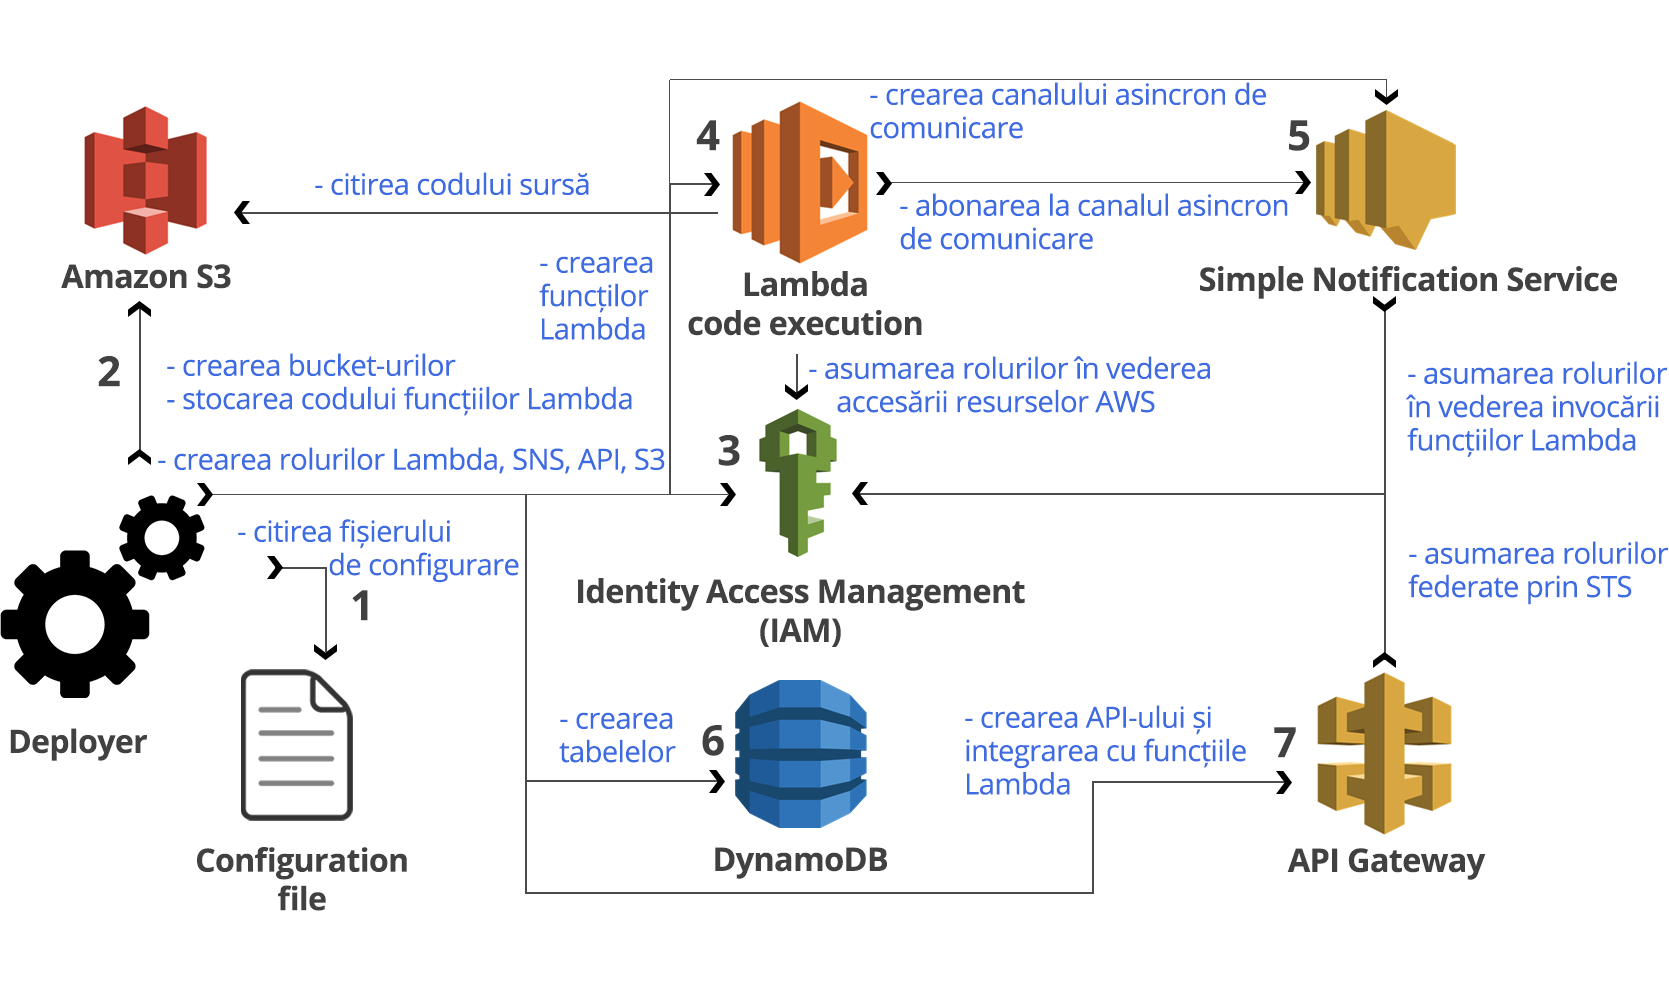
\includegraphics[keepaspectratio, width=1.0\textwidth]{generare-infrastructura.png}
	\caption{Generarea infrastructurii \cite{diagram-icons-sources}\cite{aws-icons-source}}\par\medskip 

\end{center}
\end{figure}

 
\clearpage

% Executia procesului de crawling
\section{Execuția procesului de crawling}
Această secțiune prezintă, în detaliu, modul în care aplicația "Surf" îndeplinește procesul de parcurgere a siturilor web. Mai exact, se descriu mecanismele prin care, având la dispoziție infrastructura creată cu ajutorul generatorului de resurse, utilizatorul poate beneficia de rezultatele extrase din paginile web parcurse de catre crawler. Pentru simplitate, ne vom referi la ansamblul acestor mecanisme drept un \textit{workflow}\footnote{Din engl. "workflow", care se traduce, în acest context, drept un flux de lucru, sau un proces în cadrul căruia se desfășoară o serie bine definită de activități (i.e. execuții de programe)}.
\\

\noindent
Un \textit{workflow} reprezintă unitatea de bază pe care crawler-ul web "Surf" o poate interpreta. Dintr-un \textit{workflow} se pot genera oricâte execuții. Începerea execuției unui \textit{workflow} trebuie să fie precedată de crearea acestuia. O execuție a unui \textit{workflow} întreprinde următoarele acțiuni, cu scopul parcurgerii paginilor web pentru extragerea informațiilor:

\begin{enumerate}

	\item{Preluarea, validarea și interpretarea datelor de configurare a procesului de crawling;}
	
	\item{Stocarea persistentă a definiției unei execuții a unui \textit{workflow} în baza de date, cu scopul accesării datelor necesare în contextul rulării crawler-ului;}
	
	\item{Inițializarea unui automat finit și determinist, în vederea modelării parcurgerii recursive a siturilor web în manieră \textit{breadth-first} \footnote{Parcurgea în manieră \textit{breadth-first} asigură vizitarea fiecărui nod dintr-un arbore de la adâncimea curentă, înainte de a trece la parcurgerea nodurilor de la următorul nivel de adâncime}, prin "AWS Step Functions";}
	
	\item{Crearea sarcinilor pentru parcurgerea paginilor web (\textit{taskuri}\footnote{În contextul execuției unui \textit{workflow}, un \textit{task} reprezintă o unitate de lucru, sub forma unei înregistrări în baza de date, ce poate fi preluată și executată de către un program aflat în execuție (e.g. o funcție Lambda)}), înregistrarea datelor și metadatelor rezultate în urma parcurgerii, precum și a datelor ce modelează execuția procesului de crawling (e.g. timpi maximi de răspus, adrese URL vizitate deja etc.);}
	
	\item{Distribuirea \textit{taskurilor} către funcțiile Lambda (\textit{workers}\footnote{Un \textit{worker} reprezintă un program executabil. În aplicatia "Surf", funcțiile Lambda reprezintă \textit{workerii}}) ce le vor prelua și executa;}
	
	\item{Executarea funcțiilor Lambda și stocarea/intoarcerea rezultatelor;}
	
	\item{Sincronizarea execuțiilor paralele ale funcțiilor Lambda și centralizarea rezultatelor în urma execuției \textit{task-urilor};}
	
	\item{Pornirea recursivă a unui nou \textit{workflow}, cu scopul de a parcurge un nou nivel de adâncime în procesul de crawling și de a gestiona gradul de încărcare a sistemului distribuit (e.g. respectarea limitărilor impuse de serviciile AWS, precum numărul maxim de execuții concurente ale funcțiilor Lambda în cadrul execuției unui automat "AWS Step Functions").}
	
\end{enumerate} 



\subsection{Configurare}
Pentru inceperea executiei unui workflow, este necesara, in prealabil, crearea workflow-ului. \textit{Tabelul 1} de la pagina 22 descrie datele necesare crearii unui workflow, date dintre care o parte sunt configurabile de catre utilizator (i.e. campul "Config."\footnote{prescurtare de la substantivul \textit{Configurabil}} are valoarea \textit{DA}), iar o parte sunt memorate in mod implicit odata ce workflow-ul este creat. Suita de configurari descrisa in \textit{Tabelul 1} coexista cu seria de configurari generate de creatorul de resurse. Diferenta intre cele doua consta in faptul ca generatorul de resurse defineste configurari la nivel de cont AWS. Impartirea configurarilor in doua de nivele de abstractizare (i.e. scazut pentru cele de la nivelul resurselor din contul AWS si ridicat pentru cele oferite in etapa de creare a unui workflow) confera flexibilitate in utilizarea crawler-ului "Surf". Pentru a evidentia contrastul intre cele doua configurari vom enumera, in continuare, cateva elemente esentiale ale configurarii la nivel de resurse din contul AWS:

\begin{itemize}
	\item{timpul maxim de asteptare pentru ca o cerere cloud sa fie satisfacuta;}
	\item{regiunea in care sunt create resursele AWS;}
	\item{numarul maxim de cereri pe secunda admis de catre API;}
	\item{numarul maxim de cereri pe secunda admise pentru tabelele din baza de date (configurare importanta pentru controlul costului);}
	\item{stabilirea nivelului de logare (i.e. urmarire a actiunilor utilizatorilor in cadrul interactiunii cu API-ul "Surf);}
	\item{stabilirea limbajului in care va fi generat clientul pentru API-ul creat prin API Gateway.}

\end{itemize}

\begin{table}[h]
	\centering
    \begin{tabular}{|M{2.5cm}|M{1.6cm}|M{1.25cm}|M{7.25cm}|}
    	\hline 
    	Nume camp & Tip & Config. & Descriere \\ \hline
    	
    Id & Text & NU & Id atribuit workflow-ului pentru a putea fi identificat in mod unic printre celelalte workflow-uri din tabela (din baza de date) care le gazduieste \\ \hline
    
    Data Creare & Numeric & NU & Data crearii, reprezentand numarul de milisecunde de la 1970 (engl. "epoch milliseconds") \\ \hline
    
    Proprietar & Text & NU & Identitatea atribuita utilizatorului ce a creat workflow-ul. Necesar pentru a stabili permisiuni de acces. \\ \hline
    
    Nume & Text & DA & Nume familiar atribuit workflow-ului pentru identificare facila \\ \hline
    
    Adresa Inceput & Text & DA & URL-ul de la care va porni procesul de crawling \\ \hline
    
    Selector URL & Text & DA & Expresie regulata ce valideaza daca un URL de pe o pagina vizitata de catre crawler este adaugat recursiv la lista sarcinilor pentru crawling \\ \hline
    
    Adancime maxima & Numeric & DA & Adancimea maxima la care vor fi parcurse paginile web de catre crawler (i.e. in arborele de parcurgere recursiva) \\ \hline
    
    Pagini pe nivel & Numeric & DA & Numarul maxim de pagini ce vor fi parcurse de catre crawler pe un anumit nivel de adancime (i.e. in arborele de parcurgere recursiva) \\ \hline
    
    Dimensiune maxima pagina & Numeric & DA & Dimensiunea maxima admisa (in octeti) pentru un sit web sa fie parcurs \\ \hline
    
    Grad de paralelizare & Numeric & DA & Numarul maxim de crawleri concurenti dintr-un workflow \\ \hline
    
    Politica de selectie & JSON & DA & Definitie folosita pentru a extrage date din paginile web parcurse, in functie de anumiti parametri \\ \hline
    
    Politica de reincercare & JSON & DA & Definitie folosita pentru a stabili cazurile in care incercarile esuate de a parcurge paginile web trebuie reincercate \\ \hline
    
    \end{tabular}
    \caption{Definitia unui workflow}
\end{table}
\clearpage
\clearpage

\subsection{Inițializare}
Odata ce o cerere de incepere a unei executii a unui workflow este primita de catre crawler, functia Lambda corespunzatoare inceperii executiei (i.e. \textit{"Pornire workflow"}) este invocata. Aceasta creaza si salveaza metadatele necesare in baza de date (e.g. timpul la care a inceput workflow-ul, cu scopul de a putea contoriza cat a durat executia), apoi invoca functia Lambda responsabila pentru initializarea mecanismului de distributie si sincronizare a executiei in paralel a functiilor ce parcurg paginile web. \textit{"Figura 7"} descrie modul in care functia de initializare a unui workflow este utilizata, precum si rolul pe care aceasta il indeplineste in procesul recursiv de crawling.

\begin{figure}[ht]
\begin{center}
	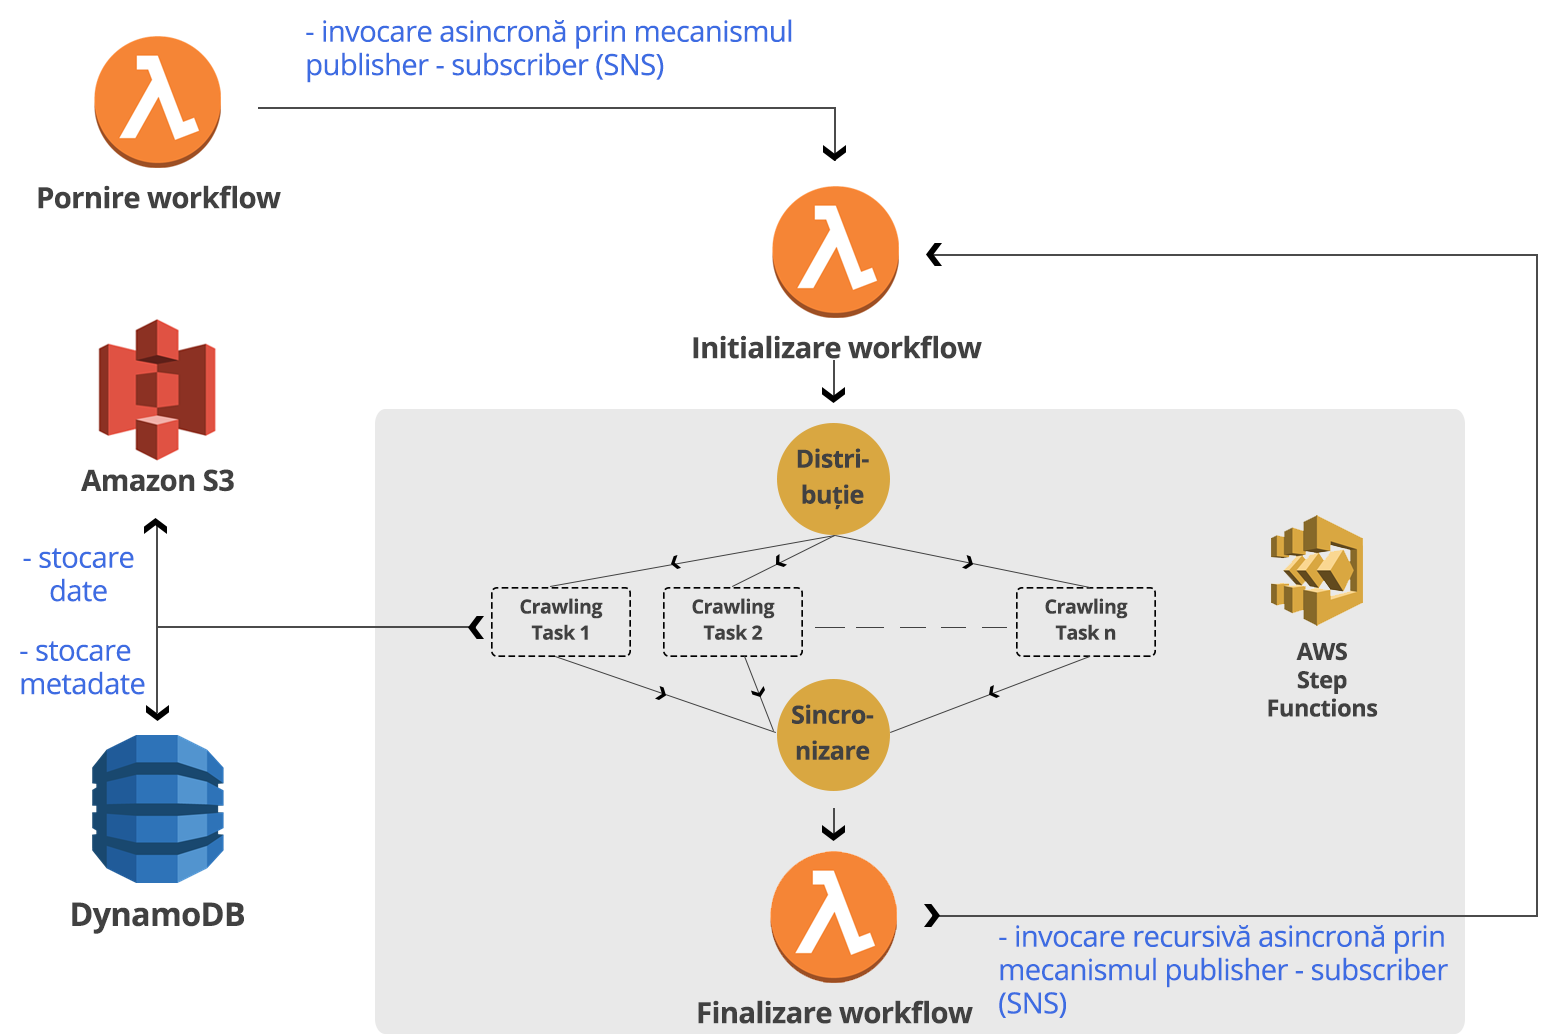
\includegraphics[keepaspectratio, width=1.0\textwidth]{proces-crawling-high-level.png}
	\caption{Arhitectura unui workflow \cite{diagram-icons-sources, aws-icons-source}}\par\medskip 

\end{center}
\end{figure}

Responsabilitatile functiei de initializare a workflow-ului sunt urmatoarele:

\begin{itemize}
	\item{Verificarea nivelului de adancime la care s-a ajuns in urma procesului de crawling si finalizarea workflow-ului, in caz ca nivelul de adancime maxim a fost depasit;}
	\item{Interogatea bazei de date in vederea extragerii task-urilor pentru parcurgerea paginilor web, task-uri ce sunt executate in cadrul automatului orchestrat de catre "AWS Step Functions";}
	\item{Crearea si pornirea automatului finit construit in cadrul "AWS Step Functions", pe baza task-urilor extrase din baza de date. Acest automat este definit prin doua stagii secventiale. Primul stagiu are ca scop orchestrarea distribuita a sarcinilor de crawling executate in paralel, iar cel de-al doilea are ca scop agregarea, interpretarea si salvarea datelor provenite din executia task-urilor concurente.}
\end{itemize}


\subsection{Parcurgere}
Functiile ce au ca scop vizitarea paginilor web sunt grupate ca stagii de executii paralele in automatul finit configurat in "AWS Step Functions". Acestea reprezinta executii ale definitiilor formale ale task-urilor de crawling. O parte dintre datele asociate unui task reprezinta metadatele configurate in pasul de creare a workflow-ului. \textit{Tabelul 2} prezinta structura unui task, cu mentiunile necesare acolo unde definitia unui camp este exact aceeasi cu definitia campului respectiv din structura unui workflow.

\begin{table}[h]
	\centering
    \begin{tabular}{|M{2.5cm}|M{1.6cm}|M{9cm}|}
    	\hline 
    	Nume camp & Tip & Descriere \\ \hline
    	
    	Id & Text & Identificator unic pentru task \\ \hline
    	
    	Id Workflow & Text & Identificatorul workflow-ului de care apartine task-ul curent \\ \hline
    	
    	Data Incepere & Numeric & Data la care a inceput executia task-ului (engl. epoch milliseconds) \\ \hline
    	
    	Data Finalizare & Numeric & Data la care s-a finalizat executia task-ului(engl. epoch milliseconds) \\ \hline
    	
    	Stare & Text & Starea in care se afla task-ul: \textit{Programat, Activ, Esuat, Depasit temporal, Intrerupt} \\ \hline
    	
		Adresa & Text & URL-ul ce trebuie vizitat in vederea extragerii datelor si metadatelor \\ \hline    	
    	
    	Adancime & Numeric & Nivelul de adancime, in arborele de parcurgere a paginilor web realizat de catre crawler, la care se afla task-ul \\ \hline
    	
    	Erori & Lista & Esecurile inregistrate in decursul executiei task-ului (ca structuri JSON) \\ \hline
    	
    	Politica de selectie & JSON & \textit{vezi Tabelul 1, pag. 22} \\ \hline
    	
    	Dimensiune maxima pagina & Numeric & \textit{vezi Tabelul 1, pag. 22} \\ \hline
    	
    	Selector URL & Text & \textit{vezi Tabelul 1, pag. 22} \\ \hline
    	
    \end{tabular}
\end{table}
\clearpage

Procesul de parcurgere a unei pagini web presupune urmatoarele etape:

\begin{enumerate}
	\item{Actualizarea starii task-ului in vederea reflectarii conditiei sale actuale (e.g. "in executie" sau "esuat");}
	
	\item{Verificarea dreptului de acces asupra URL-ului configurat in cadrul definitiei task-ului, prin consultarea fisierului robots.txt (daca acesta exista), aflat in calea de baza (engl. \textit{root}) a sitului web de la URL-ul respectiv, in concordanta cu politica de configurare a procesului de crawling;}
	
	\item{Parcurgerea sitului web:}
	\begin{enumerate}
		\item{Extragerea datelor conform politicii de selectie a datelor (configurata in pasul de creare a workflow-ului) si stocarea acestora (daca exista) in S3;}
		
		\item{Salvarea metadatelor in legatura cu datale extrase, in vederea accesarii sau cautarii facile a locatiei in care au fost salvate in S3;}
		
		\item{Selectarea tuturor legaturilor de tip URL catre alte situri web din cadrul paginii vizitate, conform politicii de urmarire a legaturilor catre alte pagini web, definita in pasul de creare a workflow-ului;}
		
		\item{Crearea de noi task-uri in starea \textit{Programat}, configurate cu un nivel de adancime superior celui pe care se afla URL-ul curent parcurs de catre crawler si salvarea acestora in baza de date, doar daca respecta configurarile declarate ca date de intrare ale executiei workflow-ului (e.g. dimensiunea maxima a unei pagini web parcurse); acest pas mai poarta denumirea de \textit{task scheduling\footnote{engl. \textit{task scheduling} = programare temporala a executiei unui task}};}
		
	\end{enumerate}
	
	\item{Actualizarea tabelei in care se tine evidenta paginilor parcurse de catre crawler in timpul executiei unui workflow, cu scopul de a nu se parcurge de doua ori acelasi URL;}
		
	\item{Prinderea, rezolvarea si stocarea erorilor survenite in cadrul procesului de parcurgere a paginilor web.}
	
\end{enumerate}

% Despre erorile in parcurgere

\subsection{Finalizare}
Procesul de finalizare a unei sesiuni de crawling are drept obiective centralizarea și analizarea datelor provenite în urma executării, în paralel, a funcțiilor responsabile pentru parcurgerea paginilor web. Responsabilitățile funcției de finalizare se pot împărți în două categorii, în funcție de motivul ce a determinat invocarea acesteia:

\begin{enumerate}
	\item{Finalizarea unei execuții îndeplinite cu succes, caz în care nu au intervenit erori extraordinare (i.e. netratate) în cadrul cel puțin unuia dintre task-urile executate în paralel;}
	\item{Finalizarea unei sesiuni de parcurgere în care au existat erori în cadrul execuției cel puțin unuia dintre task-urile executate în paralel, caz în care funcția de finalizare va îndeplini toate sarcinile ce au ramas neîndeplinite în urma terminării bruște a execuției sarcinilor paralele de crawling.}
\end{enumerate} 

\noindent
Indiferent de situația în care se află execuția worfklow-ului, funcția de finalizare a sesiunii de crawling are în vedere înregistrarea metadatelor cu privire la progresul workflow-ului (e.g. metrici Cloudwatch) și luarea deciziei conform căreia invocarea recursivă a următoarei sesiuni de crawling se face începand cu același nivel de adâncime sau cu unul superior (i.e. mai mare), în concordanță cu numarul maxim de pagini ce poate fi vizitat pe un anumit nivel de adâncime, de catre crawler.


\clearpage

% Interfata de programare
\section{Interfața de programare}
Modalitatea prin care componentele crawler-ului web "Surf" pot fi accesate, modificate si executate este reprezentata de o interfata\cite{iterface-definition} structurata sub forma unui API RESTful\footnote{engl. \textit{RESTful} = adjectiv de la abrevierea \textit{REST}; un API este \textit{RESTful} daca adopta stilul arhitectural \textit{REST\cite{rest-definition}}}. API-ul adopta stilul arhitectural REST\cite{rest-definition} deoarece acesta ajuta la decuplarea arhitecturii si simplificarea urmaririi executiei aplicatiei, prin faptul ca nu permite memorarea starilor intermediare in cadrul unei sesiuni de comunicare intre utilizator si crawler. De asemenea, API-ul RESTful confera extensibilitate si flexibilitate la nivel de interfata, intrucat permite gruparea resurselor in mod ierarhic si identificarea usoara a resurselor si a consecintelor aplicarii anumitor actiuni, prin verbe HTTP, asupra starii sistemului. \textit{"Figura 8"} prezinta secventa mimima de operatii ce trebuie efectuate, la nivel de API, pentru a putea obtine rezultate in urma procesului de parcurgere a paginilor web de catre crawler, modelate printr-o diagrama de secventa.

% Locatie creare diagrama secventa: http://gojs.net/latest/samples/sequenceDiagram.html
% Script creare diagrama secventa:
\iffalse
{ "class": "go.GraphLinksModel",
  "nodeDataArray": [
{"key":"User", "text":"Utilizator", "isGroup":true, "loc":"0 0", "duration":19},
{"key":"Api", "text":"API-ul 'Surf'", "isGroup":true, "loc":"250 0", "duration":19},
{"key":"Backend", "text":"Backend AWS", "isGroup":true, "loc":"500 0", "duration":19},
{"group":"User", "start":1, "duration":4},
{"group":"Api", "start":1, "duration":3},
{"group":"Backend", "start":2, "duration":2},
{"group":"User", "start":6, "duration":4},
{"group":"Api", "start":6, "duration":3},
{"group":"Backend", "start":7, "duration":2},
{"group":"User", "start":11, "duration":4},
{"group":"Api", "start":11, "duration":3},
{"group":"Backend", "start":12, "duration":2},
{"group":"User", "start":16, "duration":4},
{"group":"Api", "start":16, "duration":3},
{"group":"Backend", "start":17, "duration":2}
 ],
  "linkDataArray": [
{"from":"User", "to":"Api", "text":"POST /workflows", "time":1},
{"from":"Api", "to":"Backend", "text":"Validare & inregistrare workflow", "time":2},
{"from":"Backend", "to":"Api", "text":"Workflow din baza de date :id_workflow", "time":3},
{"from":"Api", "to":"User", "text":"Workflow din baza de date :id_workflow", "time":4},
{"from":"User", "to":"Api", "text":"POST /workflows/executions :id_workflow", "time":6},
{"from":"Api", "to":"Backend", "text":"Porneste workflow", "time":7},
{"from":"Backend", "to":"Api", "text":"Executie cu id :id_executie", "time":8},
{"from":"Api", "to":"User", "text":"Executie cu id :id_executie", "time":9},
{"from":"User", "to":"Api", "text":"GET /workflows/executions/:id_executie", "time":11},
{"from":"Api", "to":"Backend", "text":"Listeaza executie", "time":12},
{"from":"Backend", "to":"Api", "text":"Detalii executie", "time":13},
{"from":"Api", "to":"User", "text":"Detalii executie", "time":14},
{"from":"User", "to":"Api", "text":"GET /workflows/executions/:id_executie/metadata", "time":16},
{"from":"Api", "to":"Backend", "text":"Listeaza metadatele asociate executiei :id_executie", "time":17},
{"from":"Backend", "to":"Api", "text":"Metadate asociate cu :id_executie", "time":18},
{"from":"Api", "to":"User", "text":"Metadate asociate cu :id_executie", "time":19}
 ]}
\fi

\begin{figure}[ht]
\begin{center}
	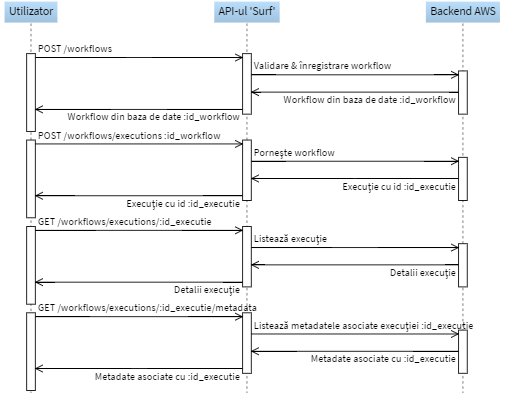
\includegraphics[keepaspectratio, width=0.9\textwidth]{diagrama-utilizator-api.png}
	\caption{Interactiunea utilizator - API \cite{diagram-icons-sources, aws-icons-source, gojs-location}}\par\medskip 

\end{center}
\end{figure}

\section{Performanță și scalabilitate}
Prin natura distribuită a crawler-ului "Surf", acesta asigură viteză în parcurgerea paginilor web şi un grad crescut de redundanţă în vederea extragerii informaţiilor din sursele selectate. Scalabilitatea orizontală\footnote{\textit{"scalabilitatea orizontală"} reprezintă posibilitatea de a adăuga mai multe maşini de lucru unui sistem informatic, pentru a-i mări performanţa} şi verticală\footnote{\textit{"scalabilitatea verticală"} se referă la posibilitatea de a îmbunătăţi performanţa maşinilor de calcul dintr-un sistem informatic, prin adăugarea de hardware mai performant} este garantată de mecanismele de scalare ale serviciilor web din cadrul Amazon Web Services.
\\ 

\noindent
Fie că este vorba despre API-ul "Surf", mecanismul asincron de notificări (SNS), asigurarea spaţiului de stocare (S3) sau funcţiile Lambda (centrul computaţional al crawler-ului "Surf"), efortul utilizatorului pentru a ajusta performanţa sistemelor menţionate constă doar în a ajusta configurările corespunzătoare serviciului care se doreşte a fi scalat\footnote{un serviciu web poate fi scalat atât în sus, adăugând putere computaţională, cât şi în jos, renunţând la putere de calcul}. În consecinţă, costurile vor varia în funcţie de gradul de performanţă care se doreşte a fi atins. Graficele de mai jos (\textit{"Figura 9"} şi \textit{"Figura 10"}) prezintă comparaţii relative între o serie variată de configurări ale sistemului cloud ce găzduieşte aplicaţia "Surf". \textit{"Figura 9"} are în vedere configuraţia \textit{"adâncime maximă: 5, număr maxim de pagini pe nivel: 30, timp de terminare sarcini maxim pentru workeri: 40 secunde, adresă de pornire: http://news.ycombinator.com/news"}. \textit{"Figura 10"} este diferită prin faptul că prezintă configuraţia \textit{"adâncime maximă: 3, număr maxim de pagini pe nivel: 100"}.
\\

\noindent
Din diagramele din figurile 9 şi 10 se poate observa faptul că gradul de paralelizare are un impact direct asupra performanţei crawler-ului. Testele s-au realizat atunci când sistemul nu era utilizat din alte motive decât cele în scopul determinării performanţei crawler-ului. Deşi este de aşteptat ca performanţa să se degradeze odată ce mai mulţi utilizatori încep să folosească serviciul de crawling "Surf", pierderea de performanţă se poate compensa crescând cantitatea de resurse alocate pentru fiecare funcţie Lambda (i.e. procesor şi memorie) şi prin configurarea tabelelor DynamoDB în vederea acceptării unui număr mai mare de cereri pe secundă.

\begin{figure}[ht]
\begin{center}
	\begin{adjustbox}{addcode={\begin{minipage}{\width}}{\caption{%
	      Performanța crawler-ului "Surf" la parcurgerile în adâncime \cite{diagram-icons-sources, aws-icons-source, microsoft-excel}
	      }\end{minipage}},rotate=90,center}
		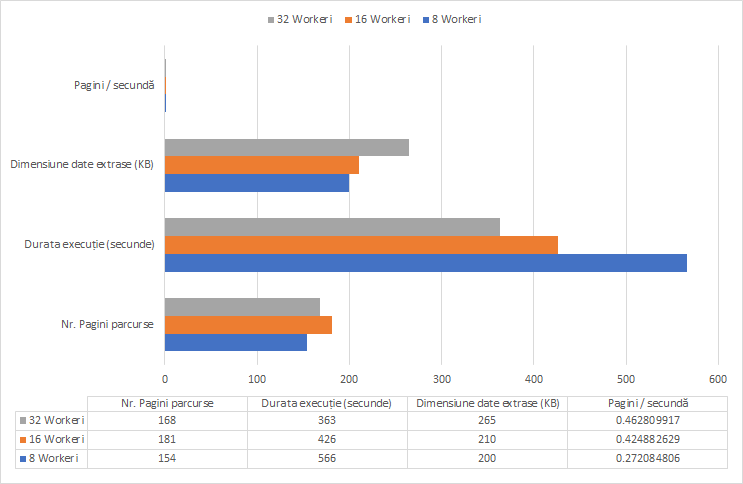
\includegraphics[keepaspectratio, scale=0.7]{depth-performance-chart.png}
	\end{adjustbox}
\end{center}
\end{figure}

\begin{figure}[ht]
\begin{center}
	\begin{adjustbox}{addcode={\begin{minipage}{\width}}{\caption{%
	      Performanța crawler-ului "Surf" la parcurgerile pe niveluri \cite{diagram-icons-sources, aws-icons-source, microsoft-excel}
	      }\end{minipage}},rotate=90,center}
	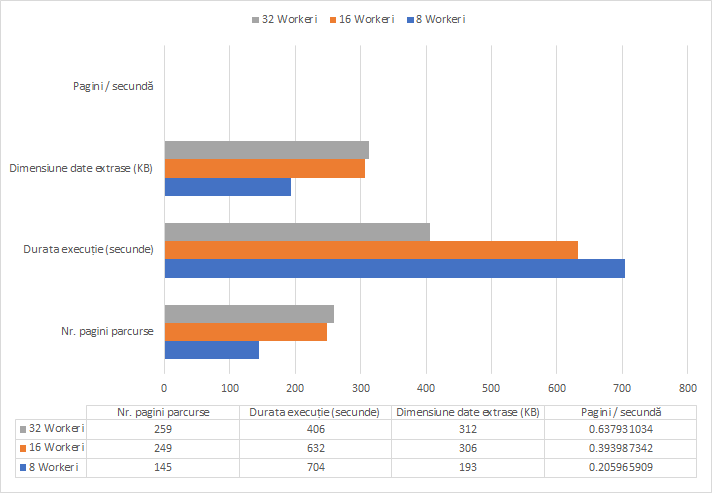
\includegraphics[keepaspectratio, scale=0.7]{breadth-performance-chart.png}
	\end{adjustbox}
\end{center}
\end{figure}


\clearpage

\section{Extensibiliate}
Pe langa facilitatile de extensibilitate oferite de utilizarea serviciilor cloud din cadrul "Amazon Web Services", arhitectura aplicatiei "Surf" prezinta urmatoarele puncte de extensie:

\begin{itemize}
	\item{Adaugare rapida si usoara de noi servicii cloud in cluster-ul aplicatiei, datorita structurii decuplate si configurabile a mecanismului de generare a infrastructurii;}
	\item{Asigurarea infrastructurii crawler-ului in mai multe regiuni globale, in conformitate cu politicile de globalizare AWS, astfel incat aplicatia "Surf" sa poata fi folosita la scara larga;}
	\item{Posibilitatea de a adauga functii Lambda de tip plug-in in cadrul mecanismului de parcurgere si procesare a informatiilor din cadrul paginilor web vizitate de catre crawler (\textit{"Figura 11"}).}
\end{itemize}

\begin{figure}[ht]
\begin{center}
	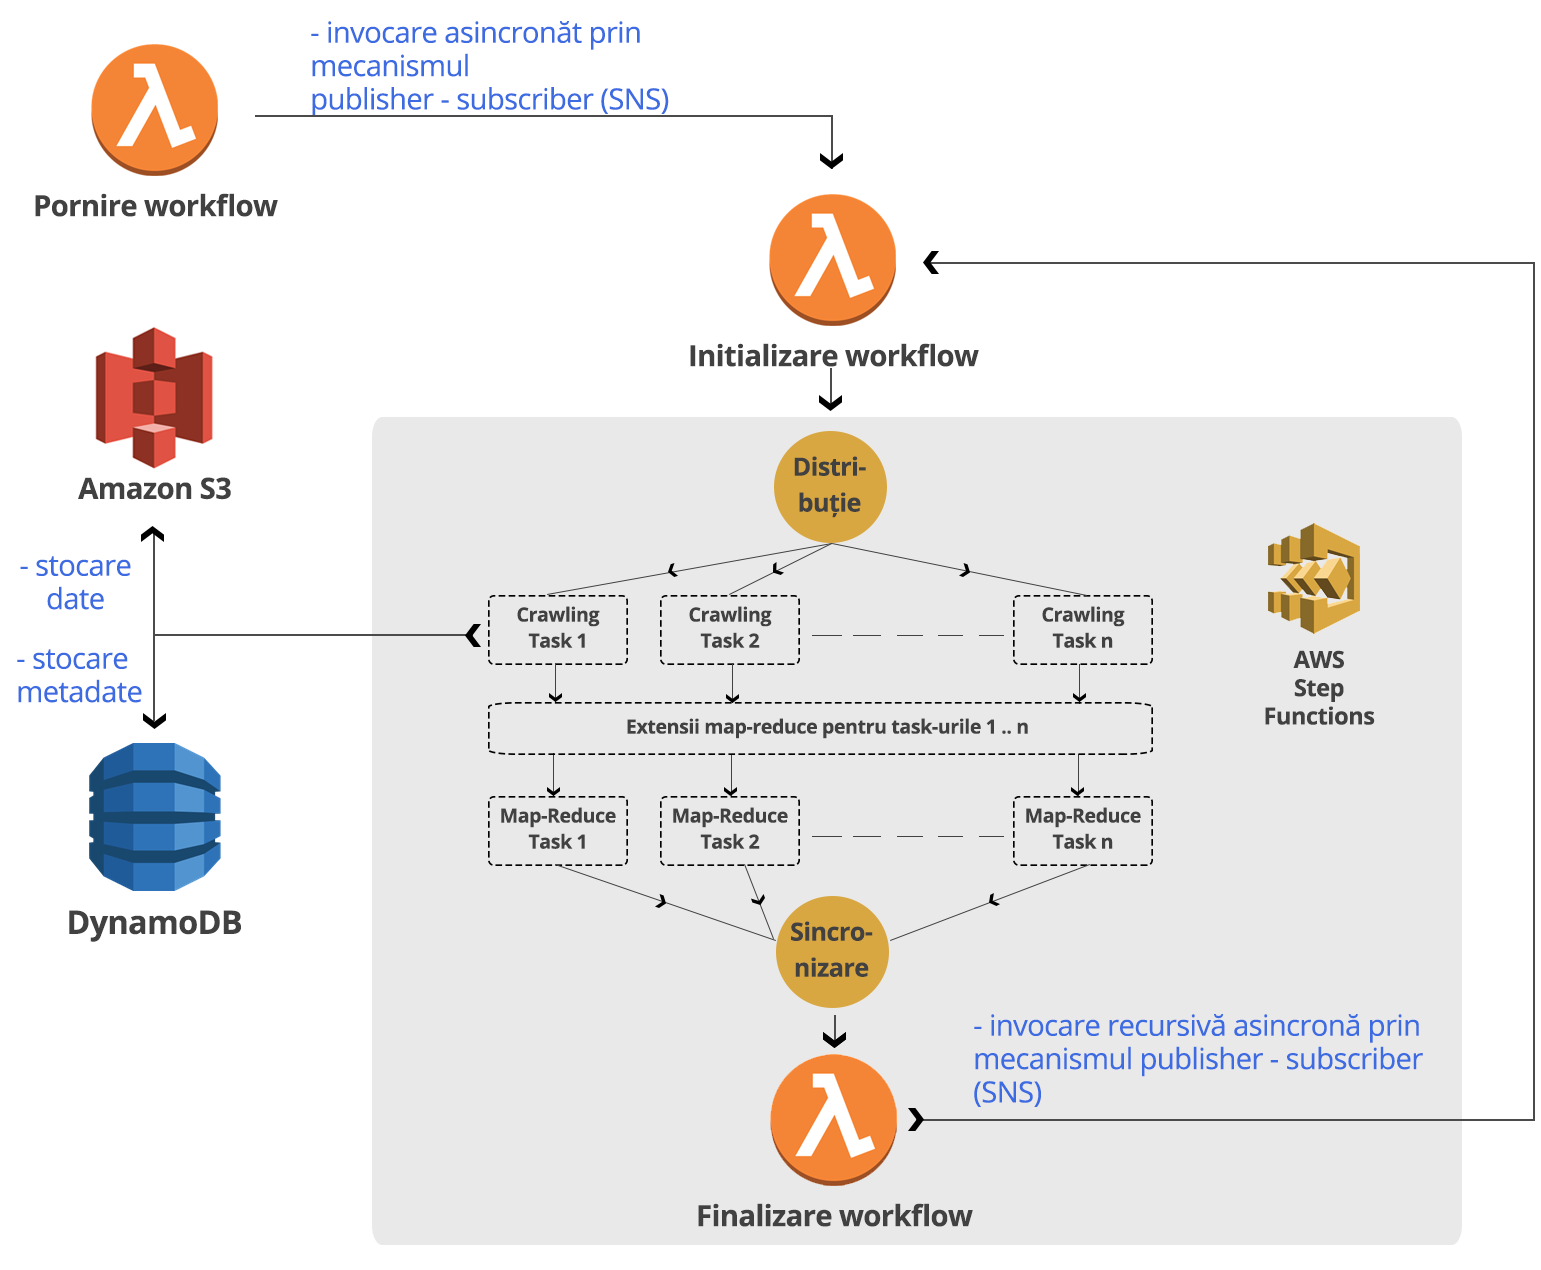
\includegraphics[keepaspectratio, width=0.9\textwidth]{proces-crawling-cu-pluginuri.png}
	\caption{Plugin-uri adaugate procesului de crawling \cite{diagram-icons-sources, aws-icons-source}}\par\medskip 

\end{center}
\end{figure}

\section{Direcții viitoare}
Aceasta sectiune prezinta, pe scurt, cateva dintre componentele proiectate pentru crawler-ul "Surf" care ar aduce avantaje reale in ceea ce priveste flexibilitatea in utilizare.

\subsection{Sistemul de plugin-uri}
Sistemul de pluginuri (prezentat, la nivel abstract, in \textit{"Figura 9"}), reprezinta o modalitate de a adauga crawler-ului web "Surf" functionalitati legate de procesarea informatiilor preluate din siturile web vizitate. Plugin-urile vor fi dezvoltate ca functii Lambda care se vor afla in contul AWS al proprietarului crawler-ului. Fiecare plugin va adera la o interfata cu scopul realizarii schimbului de informatii in cadrul automatului finit definit in cadrul "AWS Step Functions". Totodata, fiecare plugin va specifica daca, in cadrul executiei sale, vor fi salvate date si metadate in sistemele persistente de stocare. Sistemul va putea genera rezultate ale parcurgerii informatiilor din paginile web vizitate la oricare pas al executiei paralele din cadrul automatului finit, datele fiind etichetate cu prefixul functiei  care le-a generat, pentru a facilita selectarea si agregarea acestora. Cu alte cuvinte, fiecare task paralel din cadrul automatului finit va trece printr-o serie de stagii configurabile in ceea ce priveste extragerea si prelucrarea informatiilor provenite de la stagiul precedent. In cazul in care nu se doreste specificarea de plugin-uri, atunci executia taskurilor de crawling din automatul finit va avea comportamentul de baza, descris in capitolul \textit{"Crawling in cloud"}.

\subsection{Indexare periodică}
Odata ce crawler-ul web "Surf" extrage datele din paginile web vizitate, acesta creaza si o serie de metadate, cu scopul indexarii locatiei datelor in S3. Desi acest sistem functioneaza, el este limitat la accesarea datelor despre localizarea informatiilor salvate. O imbunatatire a functionalitatii aplicatiei "Surf" ar reprezenta crearea unui sistem de indexare periodica a informatiilor. Un astfel de sistem ar asigura mecanisme complexe de localizare si extragere a datelor, atat in functie de sintaxa, cat si de semantica, indeplinind urmatoarele functii:

\begin{itemize}
	\item{indexare periodica, prin mecanismul de generare de evenimente oferit de "AWS CloudWatch Events", a datelor generate in procesul de parcurgere a siturilor web;}
	
	\item{Utilizarea unui framework pentru procesarea limbajului natural\footnote{engl. "Natural language processing" pentru extragerea metadatelor referitoare la datele textuale extrase in procesul de crawling;}}
	
	\item{Utilizarea functiilor de procesare a web-ului semantic\footnote{https://www.w3.org/standards/semanticweb/} pentru a extrage, pe baza unui algoritm de clusterizare\footnote{http://www.dictionary.com/browse/clustering}, structuri semantice definitorii din paginile web vizitate\footnote{http://schema.org/}.}	
	
\end{itemize}

Odata grupate si generate, datele ce alcatuiesc mecanismul de indexare pot fi clasificate utilizand algoritmi de clasificare probabilista, pentru a restrage spatiul de cautare atunci cand se recurge la cuvinte cheie.

\subsection{Sistemul de notificări}
În funcție de preferințele utilizatorilor, aplicația "Surf" poate fi dezvoltată în direcția configurării execuțiilor periodice pe bază de evenimente generate în cloud (e.g. expresii CRON\footnote{https://docs.oracle.com/cd/E12058\_01/doc/doc.1014/e12030/cron\_expressions.htm} în cadrul CloudWatch Events). În acest caz, este necesar un sistem de notificări asincrone care să îi înștiințeze pe utilizatori despre progresul pe care crawler-ul îl face în decursul execuției unui workflow. Flexibilitatea sistemului cloud din cadrul "Amazon Web Services" permite utilizarea de mecanisme multiple pentru a transmite notificări precum:

\begin{itemize}

	\item{\textit{Simple Notification Service:} permite transmiterea de notificări prin mecanismul publisher-subscriber\footnote{https://docs.oracle.com/cd/B10501\_01/appdev.920/a96590/adg15pub.htm}; notificările pot fi configurate pentru o gamă largă de destinații, de la adrese de e-mail, până la notificări \textit{push} adresate sistemelor de operare mobile;}
	
	\item{\textit{Simple Email Service:} permite trimiterea de e-mailuri către utilizatori; e-mailurile pot fi configurate astfel încât să accepte limbaj de markup avansat, redând o experiență mai bogată utilizatorilor.}
	
\end{itemize}


\clearpage

\setcounter{section}{0}
\chapter*{\chaptertitle{Contribuții personale}}
\addcontentsline{toc}{chapter}{Contribuții personale}
Crawler-ul web "Surf" prezintă următoarele caracteristici cheie în ceea ce priveşte dezvoltarea, rularea şi mentenanţa unui crawler web distribuit:

\begin{itemize}

	\item{Are capacitatea de a-şi genera fiecare resursă necesară, utilizând programul definit ca \textit{"Generator de resurse"}. Această funcţionalitate permite crawler-ului să fie construit în cadrul oricărui cont "Amazon Web Services", într-o regiune globală pe care utilizatorul o poate configura. Totodată, se permite administratorului financiar al contului AWS să aibă un control fin asupra costurilor generate de către crawler, deoarece limitele rezervate serviciilor web folosite de către crawler pot fi configurate în mod individual;}

	\item{Permite integrarea cu un sistem de autentificare sigur, bazat pe federearea identității web în raport cu un furnizor terţ de identităţi de încredere. În urma autentificării, crawler-ul web "Surf" asigură autorizarea cererilor într-o manieră flexibilă, bazată pe documente ce definesc politici de securitate. Odată autorizaţi, utilizatorilor le sunt alocate chei de acces asupra API-ului, care stabilesc limite configurabile asupra numărului de cereri pe secundă pe care aceştia le pot efectua;}

	\item{Oferă scalabilitate orizontală şi verticală, atât în sus cât şi în jos, în ceea ce priveşte mecanismul de parcurgere concurentă a paginilor web, prin stabilirea, în cadrul fiecărui workflow, a unui grad de paralelizare menit să se adapteze cerinţelor de timp şi cost ale fiecărui utilizator;}

	\item{Poate fi distribuit drept un executabil care să creeze, având definit, în prealabil, un fişier de configurare, într-un interval de aproximativ două minute, toată infrastructura AWS necesară utilizării aplicaţiei cu scopul de a parcurge paginile web pentru a extrage informaţii;}

	\item{Oferă, pentru dezvoltatori, o interfaţă de programare flexibilă şi prietenoasă, ce respectă stilul arhitectural REST; De asemenea, permite dezvoltatorilor posibilitatea de a integra alte servicii cloud din cadrul AWS pentru a extinde funcţionalităţile crawler-ului.}

\end{itemize}


\setcounter{section}{0}
\chapter*{\chaptertitle{Concluzii}}
\addcontentsline{toc}{chapter}{Concluzii}
Datorită ritmului alert în care se creează sau schimbă informaţiile aparţinând world wide web-ului, există o necesitate tot mai mare de a putea prelua şi analiza datele într-un mod automat, rapid şi eficient. Crawlerii web sunt o componentă deosebit de importantă, în vederea extragerii şi indexării exhaustive a informaţiilor, pentru motoarele de căutare. Cu toate acestea, avantajele aduse de către crawleri pot fi folosite şi pentru a extrage resurse relevante dintr-un anumit context, fără a fi necesară o parcurgere a tuturor resurselor web accesibile. Odată cu apariţia şi dezvoltarea serviciilor web, infrastructura puternică şi costurile reduse oferite de către furnizorii cloud oferă modalităţi flexibile, intuitive şi extensibile de a susţine crawleri specializaţi. 
\\

\noindent
Crawler-ul web "Surf" propune, în acest sens, o modalitate simplă pentru ca un utilizator interesat de resurse dintr-o anumită arie să poată să le preia automat şi să le analizeze conţinutul, fără a fi necesar să depindă de furnizori terţi de servicii web de crawling şi cu posibilitatea de ajustare minuţioasă a costurilor operaţionale. Paralelizarea sarcinilor de parcurgere a paginilor web, împreună cu scalabilitatea orizontală şi verticală asigurată de servciile cloud, garantează adaptabilitatea aplicaţiei "Surf" la cele mai diverse nevoi ale utilizatorilor săi. Flexibilitatea legată atât de costuri, cât şi de design-ul arhitectural al aplicaţiei "Surf" alături de API-ul RESTful, care expune funcţionalităţile într-un mod accesibil şi extensibil, permite dezvoltatorilor interesaţi să adauge elemente suplimentare, precum: componente de tip map/reduce, analiză semantică a conţinutului paginilor web şi tehnici euristice pentru selectarea frontierei de URL-uri. De asemenea, flexibilitatea serviciilor cloud garantează atingerea unui nivel de activitate de aproape 100\%, oferind siguranţă şi încredere în utilizare.


\clearpage

% Bibliografie
\begin{thebibliography}{99}

\bibitem{cisco-internet-traffic}
"Visual Networking Index", Cisco Systems
  
\bibitem{http://www.internetlivestats.com/total-number-of-websites/}
http://www.internetlivestats.com/total-number-of-websites/

\bibitem{ShkapenyukSuel} 
Vladislav Shkapenyuk and Torsten Suel.
\textit{Design and Implementation of a High-Performance Distributed Web Crawler}.\\
\texttt{http://cis.poly.edu/tr/tr-cis-2001-03.pdf}

\bibitem{Pantil} 
Yugandhara Patil and Sonal Patil.
\textit{Review of Web Crawlers with Specification and Working}.\\
\texttt{http://www.ijarcce.com/upload/2016/january-16/IJARCCE\%2052.pdf}

\bibitem{GautamPadminiFilippo} 
Pant Gautam, Srinivasan Padmini and Menczer Filippo.
\textit{Crawling the Web}.\\
\texttt{https://pdfs.semanticscholar.org/a4f4/5f3a3d7d53a40b7b2579392a5db88cc1b822.pdf}

\bibitem{PantSrinivasanMenczer} 
Pant Gautam, Srinivasan Padmini and Menczer Filippo.
\textit{Exploration versus exploitation in topic driven crawlers}.\\
\texttt{$https://www.researchgate.net/publication/2946755_Exploration_versus_Exploitation_in_Topic_Driven_Crawlers$}

\bibitem{StochasticModels} 
S. Ravi Kumar, P. Raghavan, S. Rajagopalan, D. Sivakumar, A. Tomkins, and E. Upfal.
\textit{Stochastic models for the Web graph}.\\
\texttt{http://cs.brown.edu/research/webagent/focs-2000.pdf}

\bibitem{RobotsStandard} 
Martijn Koster.
\textit{A Standard for Robot Exclusion}.\\
\texttt{http://www.robotstxt.org/orig.html}
  
\bibitem{web-crawler-selection-policy}
http://www.cellopoint.com/media\_resources/blogs/2011/03/Web\_Crawlers

\bibitem{distribution-of-crawling-tasks}
http://cis.poly.edu/tr/tr-cis-2001-03.pdf

\bibitem{serverless-characterization}
Miller, Ron (24 Nov 2015). "AWS Lambda Makes Serverless Applications A Reality". TechCrunch. Retrieved 10 July 2016.

\bibitem{diagram-icons-sources}
Sursele pictogramelor includ \emph{https://www.iconfinder.com} si \emph{http://simpleicon.com}.

\bibitem{aws-icons-source}
Sursa pictogramelor asociate "Amazon Web Services": \emph{https://aws.amazon.com/architecture/icons/}

\bibitem{iterface-definition}
Definitia cuvantului \textit{interfata} a fost adaptata pornind de la definitia de la adresa \emph{https://www.merriam-webster.com/dictionary/interface}

\bibitem{rest-definition}
\emph{http://www.ics.uci.edu/~fielding/pubs/dissertation/rest\_arch\_style.htm}

\bibitem{gojs-location}
Diagrama de secventa a fost generata folosind API-ul aflat la adresa \emph{http://gojs.net/latest/samples/sequenceDiagram.html}

\bibitem{microsoft-excel}
Diagramele au fost realizate utilizand programul "Microsoft Excel" (\emph{https://products.office.com/ro-ro/excel})

\end{thebibliography}

\end{document}
